\documentclass[msc,lith,english]{liuthesis}

% Settings go in settings.tex
%%% settings.tex --- 
%% 
%% Filename: settings.tex
%% Description: 
%% Author: Ola Leifler
%% Maintainer: 
%% Created: Tue Oct 19 21:11:31 2010 (CEST)
%% Version: $Id$
%% Version: 
%% Last-Updated: Tue Apr 25 08:49:48 2017 (+0200)
%%           By: Ola Leifler
%%     Update #: 43
%% URL: 
%% Keywords: 
%% Compatibility: 
%% 
%%%%%%%%%%%%%%%%%%%%%%%%%%%%%%%%%%%%%%%%%%%%%%%%%%%%%%%%%%%%%%%%%%%%%%
%% 
%%% Commentary: 
%% 
%% 
%% 
%%%%%%%%%%%%%%%%%%%%%%%%%%%%%%%%%%%%%%%%%%%%%%%%%%%%%%%%%%%%%%%%%%%%%%
%% 
%%% Change log:
%% 
%% 
%% RCS $Log$
%%%%%%%%%%%%%%%%%%%%%%%%%%%%%%%%%%%%%%%%%%%%%%%%%%%%%%%%%%%%%%%%%%%%%%
%% 
%%% Code:

\usepackage[backend=biber,hyperref]{biblatex}
%% To set the font of your thesis, use the \setmainfont{} command,
%% surrounded with \ifxetex if you want to switch between xelatex and pdflatex
\ifxetex 
%\setmainfont [Scale=1]{Georgia}
\fi

%%%%%%%%%%%%
%% The VZ43 chapter style, from Memoir contributed chapter styles: ftp://ftp.tex.ac.uk/ctan%3A/info/MemoirChapStyles/MemoirChapStyles.pdf
%%%%%%%%%%%

\usepackage{calc,color}
\newif\ifNoChapNumber
\newcommand\Vlines{%
\def\VL{\rule[-2cm]{1pt}{5cm}\hspace{1mm}\relax}
\VL\VL\VL\VL\VL\VL\VL}
\makeatletter
\setlength\midchapskip{0pt}
\makechapterstyle{VZ43}{
\renewcommand\chapternamenum{}
\renewcommand\printchaptername{}
\renewcommand\printchapternum{}

\renewcommand\chapnumfont{\Huge\bfseries\centering}
\renewcommand\chaptitlefont{\Huge\bfseries\raggedright}
\renewcommand\printchaptertitle[1]{%
\Vlines\hspace*{-2em}%
\begin{tabular}{@{}p{1cm} p{\textwidth-3cm}}%
\ifNoChapNumber\relax\else%
\colorbox{black}{\color{white}%
\makebox[.8cm]{\chapnumfont\strut \thechapter}}
\fi
& \chaptitlefont ##1
\end{tabular}
\NoChapNumberfalse
}
\renewcommand\printchapternonum{\NoChapNumbertrue}
}
\makeatother


%% To set bibliography options, refer to the biblatex manual and use
%% the ExecuteBibliographyOptions command below to set your options

\ExecuteBibliographyOptions{maxnames=99}


%% Change this to your appropriate BibTeX reference file (.bib)

\addbibresource{references.bib}

%%%%%%%%%%%%%%%%%%%%%%%%%%%%%%%%%%%%%%%%%%%%%%%%%%%%%%%%%%%%%%%%%%%%%%
%%% settings.tex ends here

%%% Local Variables: 
%%% mode: latex
%%% TeX-master: "demothesis"
%%% End: 

\usepackage{rotating}
\usepackage{color}
\usepackage{caption,subcaption}

% \usepackage{changebar}

\department{Institutionen för datavetenskap}
\departmentenglish{Department of Computer and Information Science}
\departmentshort{IDA}

% Include an external supervisor on the cover page
\externalsupervisor{Mikael Nilsson}
\supervisor{Marco Kuhlmann}
\examiner{Arne Jönsson}
\titleenglish{Labelling Clinical Reports by Exploiting the Data Structure Through Topic Modelling and Active Learning}
%\subtitleenglish{with a subtitle}
\titleswedish{Uppmärkning av kliniska rapporter genom att utnyttja strukturen hos datan med topic modeller och active learning}
\thesissubject{Datavetenskap}

\publicationyear{2018}
\currentyearthesisnumber{001}
\dateofpublication{2018-06-08}

\author{Simon Lindblad}

\newcommand{\thirdsubfig}[2]{
    \begin{subfigure}[b]{0.3\textwidth}
        \centering
        \fbox{\includegraphics[width=4cm]{figures/#1.eps}}
        \caption{#2}
        \label{subfig:#1}
    \end{subfigure}
}
\begin{document}

\chapterstyle{VZ43}

\chapter{Introduction}
\label{cha:introduction}

The world's population is growing each year. 
In order to raise to the challenges that arise with a growing population, it is of great importance that healthcare is made to be more efficient and robust.
One way of increasing the efficiency as well as the quality of healthcare is to create automated systems that can aid doctors in their process.
As the population grows, it is of utmost importance to ensure that the quality of diagnoses remain high, and that the risk of missing some critical piece of information is minimized.
Taking advantage of the available medical information is key to create such systems.

Most of the approaches that exists today to create the aforementioned automated systems need a set of categorized data in order to identify and exploit certain patterns.
The purpose of this thesis is to evaluate different techniques for labeling multi-label clinical reports.
The goal is to make the set of labeled reports more useful in future systems by labeling them based on a strategy instead of selecting them at random.
By using a selection strategy, the need for a large set of labeled reports could be reduced.
The work is done at Sectra Medical Imaging IT Solutions AB in connection with a research project they have with Region Skåne.
Region Skåne is responsible for the healthcare in Skåne, the southern most county of Sweden.
This research project project on investigating how to use machine learning and text mining techniques to improve the functionality of their products and aid the physicians in their work.

\section{Motivation}
\label{sec:motivation}

Information pertaining to a patient's diagnosis is often in the form of written clinical reports.
This is a good example of data that can be utilized in automated systems.
By extracting information from old reports, the process of writing new ones can be simplified.
A system could show cases with similar features as the one currently being written, the doctor could then compare the findings and check if they have obtained an abnormal result.
Being able to perform such a comparison will result in extra quality assurance in the diagnostic flow.
It could also provide doctors with more confidence in that their diagnosis is correct.

The problem systems like this would face is to categorize medical reports in order to make further suggestions.
One approach that is commonly used for such problems is machine learning, which is a field where a set of inputs is used to create a mapping to some output values~\cite{bishop2006pattern}.
This is done by using data to build a, usually statistical, model.

The task of predicting a category, or class, for a given text document is called text classification.
Text classification is usually solved using supervised learning~\cite{aggarwal2012surveyclass}. 
In supervised classification, there exists a set of inputs, in this case text data, that already have a category assigned to them.
This data is then used to fit the model so that it later can make predictions for inputs that it has not yet been exposed to.
Some models that have been shown to be successful in text classification are Neural Networks, Bayesian Classifiers, Decision Trees and Support Vector Machines (SVM)~\cite{aggarwal2012surveyclass,joachims1998text, aggarwal2012surveyclass, tong2001support}.

In order to fit a machine learning model to predict categories for clinical reports, we need a set of already categorized data.
That is, categories need to be assigned to an existing set of clinical reports.
It is often the case that text data is widely available.
Coming by data that is already categorized is on the other hand much harder.
Obtaining high quality data is important for use in machine learning systems, both in healthcare and in other areas.

Since the models require a sufficient amount of categorized reports, the task of categorizing them can be cumbersome.
Improving the categorization is especially important in the case of clinical data, since doctors and other clinicians time is both valuable and expensive.
By improving the process and the quality of data to be labeled, and thereby reducing the number of reports that need to be categorized, they can spend more time doing their job.

Assigning categories to reports is often referred to as labeling.
A field within machine learning that is focused on the task of improving the data labeling process is called active learning.
It is a form of semi-supervised learning.
The algorithm queries an oracle (in this case a doctor) for labels for the data points that it thinks will help the model improve the most.
An overview of the components in an active learning system can be seen in Figure~\ref{fig:active-learning-model}.
This is used when there is plenty of readily available data, but assigning labels is expensive.
Since the data points to be labeled are actively selected, the model can require fewer examples than if they were selected at random.
The points can be selected by considering the certainty of the models, and request to label the documents that the model is less certain about.
Another approach, which has not been given as much attention, is using the underlying structure of the data to select points.
The goal with this approach is to capture the distribution of the categories by applying techniques such as clustering.

\begin{figure}
    \centering
    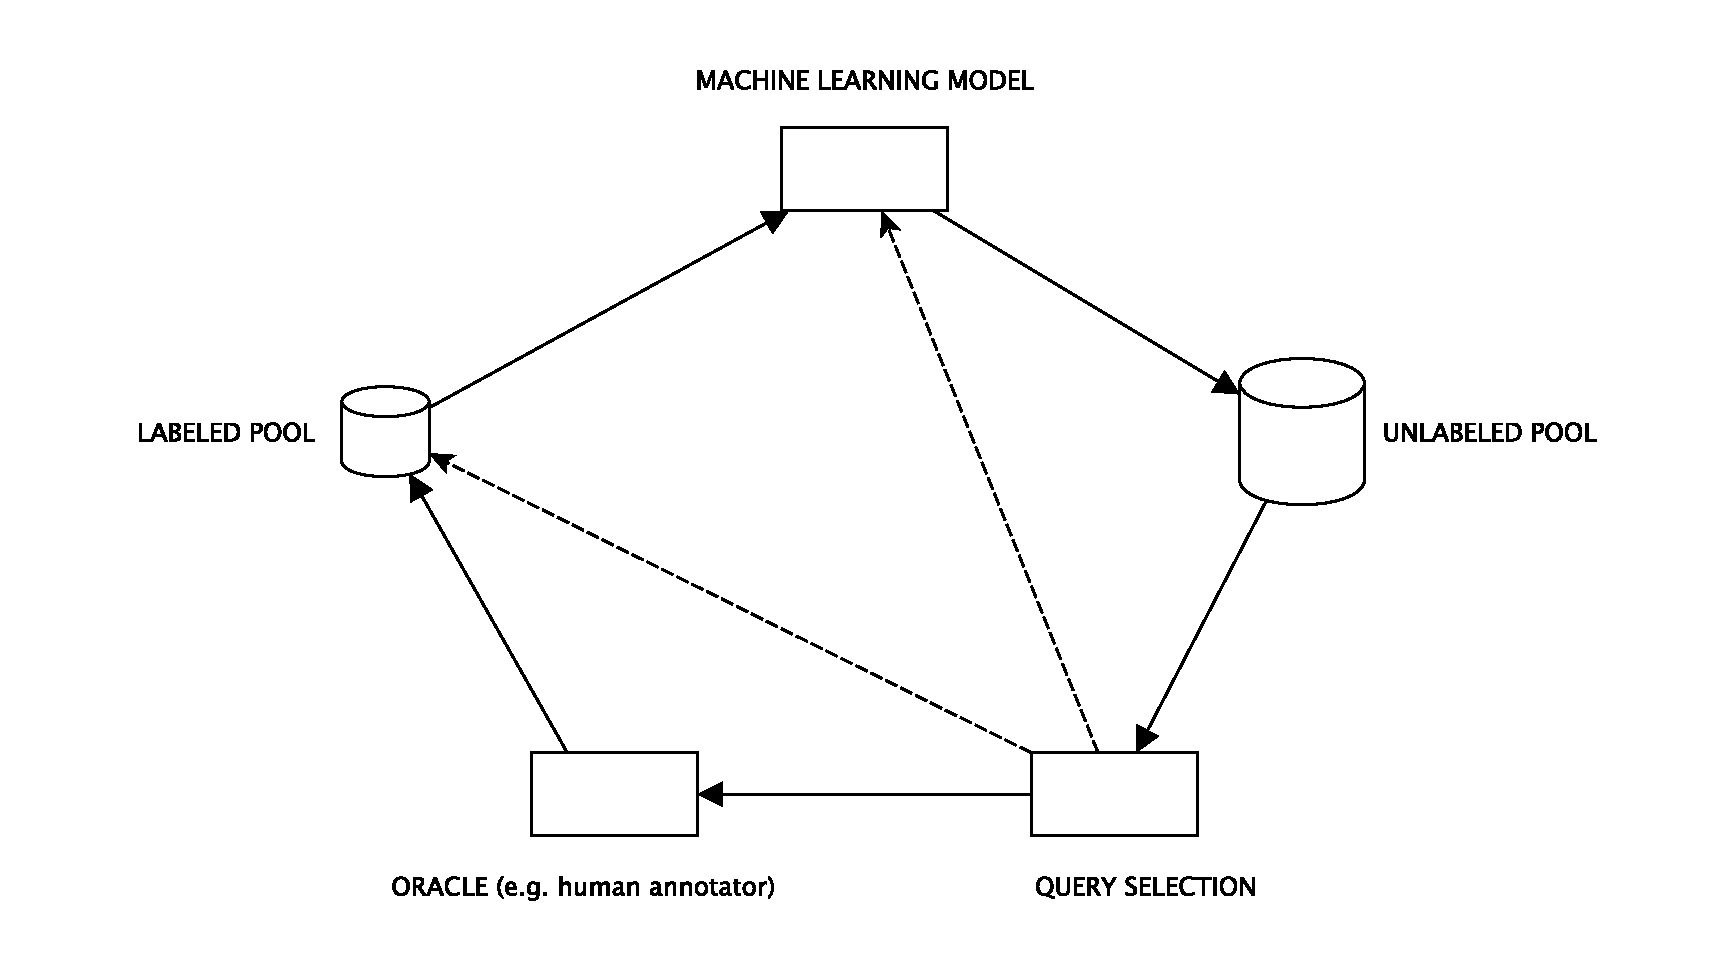
\includegraphics[width=\textwidth]{figures/active-learning-model.eps}
    \caption{An overview of an active learning system. The dotted lines represents the things that some samplings strategies base their calculations on.}
    \label{fig:active-learning-model}
\end{figure}

If one of two categories is assigned to each document, it is called a binary classification problem~\cite{bishop2006pattern}.
Problems where one of several classes is assigned to an instance are called a multi-class classification problem.
Multi-labeled classification is when one or more categories are assigned to each document.
This thesis is mainly concerned with the multi-label case.
Assigning several categories to a document is more time consuming than in the cases where only one option needs to be identified.
In those cases the process can be stopped when the appropriate category has been found.
However, when a document can be assigned several categories, the entirety of the text needs to be considered.
For example, a news article can be on several subjects, such as both economics and sport.
Even when the category sport has already been identified, the rest of the document still has to be read in order to find any additional categories.
Using active learning to enhance the labeling of documents is therefore even more useful in the multi-labeled case, since the cost of labeling the individual reports is higher.

\section{Aim}
\label{sec:aim}

The purpose with this thesis project is to evaluate different active learning techniques that can be used to increase the quality of the labeled reports.
Increasing the quality of the reports will also reduce the need for a large set of labeled reports within the project.
Resulting from this will be a complete, standalone, system for labeling reports.
The reports are interactively queried so a user can label the ones that are deemed most useful by the system.
Labeling data to use in machine learning will probably be necessary for a long time ahead, but the aim here is to create a system that makes it more efficient.
The technique chosen will then be used together with an existing web interface that Sectra created for the purpose of labeling reports.
The existing web interface can be seen in Figure~\ref{fig:web-interface}.

\begin{figure}
      \centering
      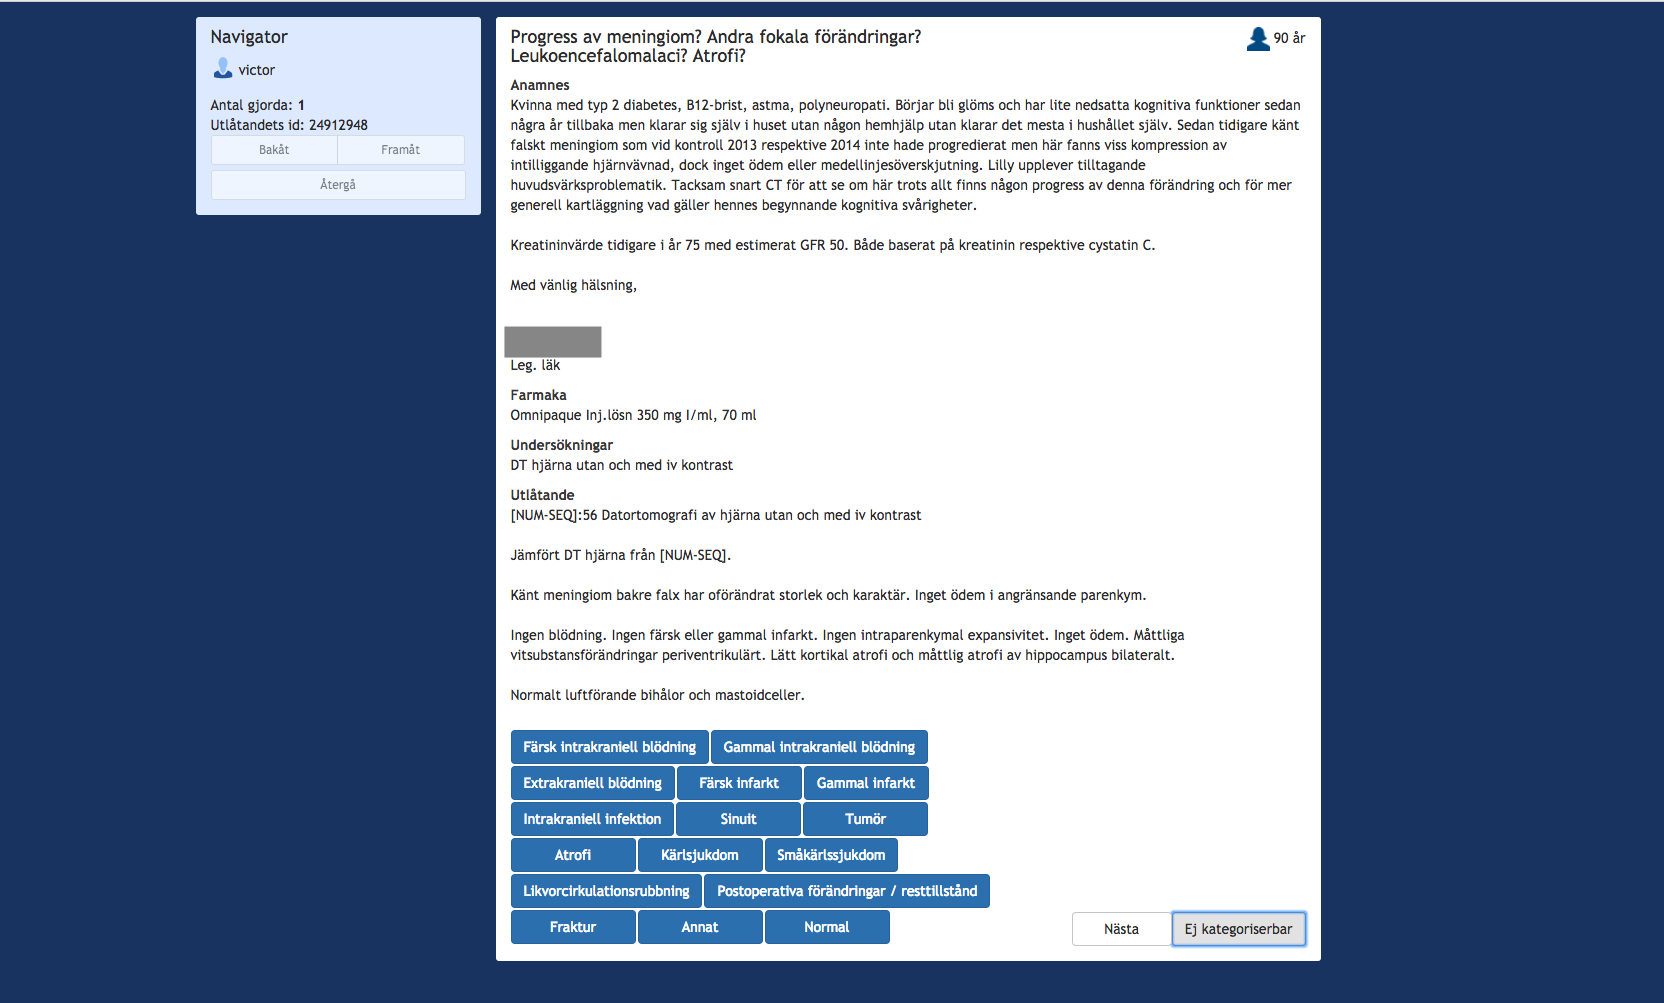
\includegraphics[width=\textwidth]{web-interface}
      \caption{A screenshot of the interface used to label clinical reports at Sectra. 
               A report is presented to the user, who can then select whichever categories (the blue buttons) deemed appropriate.
               By pressing ``next'', the system presents a new reports.}
      \label{fig:web-interface}
\end{figure}

In the work that they have done so far in the research project a doctor has labeled an initial set of reports.
This was done by simply selecting the reports in the order they were on file.
The doctor that primarily worked with the labeling stated that the distribution over the labeled categories was very skewed.
The vast majority of labeled documents were assigned to a small subset of the categories.
A skewed dataset causes the number of clinical reports that need to be labeled to increase a lot.
For a statistical model to be able to achieve good results with the less frequently occurring categories, a large number of reports needs to be labeled in order to obtain a good amount of reports with these categories.
Obtaining a more balanced dataset is desirable.

In addition to this, the doctors had come up with a new set of labels that were to be used.
So the query strategies have to work from a non-existent, or very small, initial set of labeled reports.

\section{Research questions}
\label{sec:research-questions}

The specific research questions that this thesis treat are presented here.
They are the main focus of study.
There are two main research questions, both of which relate to active learning.
In addition to this, a question regarding how to remove reports that does not need to be labeled is treated as well.

The clinical reports are of a multi-label nature.
How we are choosing the documents to be sampled is important.
Three different query strategies for active learning are evaluated for this purpose.
These are: binary version space minimization, maximum loss reduction with maximum confidence and adaptive active learning.
Their properties will be described in Chapter~\ref{cha:theory}, and a motivation behind the choice of strategies will be made in Chapter~\ref{cha:discussion}.
The algorithms to be evaluated will be based on the models certainty, as well as taking advantage of the underlying structure of the data through clustering.
The first two questions treats the evaluation of the different strategies.

\begin{enumerate}
      \item \label{intro:re-q1} 
      \textit{How well does a machine learning model perform on the dataset provided by the data, given the constraints of the project?}
      \newline
      If the decision boundaries of the models can be used to pick documents that would be more informative for the model, the number of labeled documents could hopefully be reduced while still obtaining the same performance.
      When choosing the algorithm to use in the final system, there are several different constraints that will affect the final results, and therefore need to be taken into consideration.
      The number of initial reports needed for the strategies need to perform well, and the how many labeled samples need to be acquired to achieve good results will therefore be taken into account.
      In this regard, the strategies will be evaluated based on how well an SVM model perform on the data provided by them.
      This evaluation will be based on the accuracy, precision, recall and $F_1$-score of the model.
      The labeling application is running on limited hardware, so the time it takes to run the strategies will also be evaluated.

      \item \label{intro:re-q2}
      \textit{How do the the strategies affect the balance of labels in the labeled dataset?}
      Another indication on the quality of the labeled reports is the balance between the classes.
      Based on the initial sampling, the underlying distribution of labels in the clinical data is far from uniform.
      There are certain categories, like the one describing that everything is okay with the patient, that are a lot more common than other more rare illnesses.

      If the dataset that is being sampled is skewed, i.e. some categories are a more frequent than others, our labeled set will likely follow that distribution.
      This will result in models requiring a lot of labeled documents to gather a sufficient amount of reports that are of the less common categories.
      Without these, the model with only perform well on the frequently occurring categories.
      Even though the original data may be imbalanced, selecting samples that contain a better balance between the different categories could improve the performance of the models.
      When a training set is imbalanced, the standard learning algorithms' performance can be significantly reduced~\cite{he2009learning}.
      The goal here is to see which one of the different sampling techniques that will result in the best balance between the different categories in the resulting dataset.

\end{enumerate}

In addition to this, after exploring the data it became clear that a substantial amount of reports states that an examination did not occur.
There was no standard format to these, but their subject matter was very similar the third research question treats whether or not these reports can be filtered out using unsupervised machine learning techniques.

\begin{enumerate}
      \setcounter{enumi}{2}
      \item \label{intro:re-q3}
      \textit{To what degree is it possible to filter out invalid clinical reports by using an unsupervised techniques such as topic modeling?}
      \newline
      In the dataset from Sectra, there are reports describing patients not showing up for, or changing the time of their appointments, deceased patients or patients that have been ordered to go to another hospital.
      These reports do not contain any information of value from a medical point of view and should be discarded in the labeling process.

      Unsupervised machine learning models such as topic modeling do by definition not require any labeled documents to train on.
      If it is possible to, without any such data, to capture the necessary variance and group these invalid reports together and they can be removed from the labeling process before a doctor is presented with them.
      That would result in an additional hurdle being removed from the process.
      The filtering of reports will be evaluated using  accuracy, precision, recall and $F_1$-score.
\end{enumerate}

\section{Delimitations}
\label{sec:delimitations}

The active learning techniques will be evaluated on the publicly available Reuters dataset.
Even though the sampling strategies are evaluated objectively on this, the applicability of the techniques on clinical data is only evaluated by one physician.
That part of the study is therefore inherently subjective.
Another limitation to this evaluation is that it is performed on the dataset provided by Sectra, which is not available for public use, so any conclusions drawn from it may not be applicable in other scenarios.

\section{Structure of the Report}
\label{sec:structure}

Chapter~\ref{cha:theory} covers the theory behind the different active learning strategies used, as well as some techniques used for classification and processing of text.
After this, the data and an analysis of it is described in chapter~\ref{cha:data}, which is followed by Chapter~\ref{cha:experiements}, which presents the different experiments as well as their results.
The method and results are then discussed in Chapter~\ref{cha:discussion}.
Finally, Chapter~\ref{cha:conclusion} presents the conclusions and answers the research questions.

\chapter{Theory}
\label{cha:theory}

In this chapter, the theory behind the techniques used in this thesis work is presented.
The first section treats supervised text classification, which acts as a foundation for the active learning that comes after.
Active learning is the main focus of the chapter, and an overview of the field as well as some concrete techniques is covered.
The techniques are mainly in regard to multi-labeled data.
In addition to this, some unsupervised methods used in the data processing is presented.
This chapter ends by going through the different evaluation metrics that are be used to assess the methods used.

Most of this Chapter deals with text data.
Before using the techniques presented in this chapter, the text needs to be represented in a way that is easy to work with.
\textit{Bag-of-words} (BoW) is one of the more common representations when performing text analysis. 
Using BoW the text is represented as a multi-set, a document is represented by the number of occurrences of the different words. 
Like the name implies, the positions of the words are not taken into account, they are viewed as if they were taken from a bag. 
One way to incorporate positional information into the representation is the use of n-grams.
Instead of storing information pertaining to one term, information is stored with regards to n consecutive terms.
Consider the text ``Pattern Recognition and Machine Learning''.
The use of an n-gram with n=2, called a bigram, would result in the tokens: ``Pattern Recognition'', ``Recognition and'', ``and Machine'', and ``Machine Learning''.

\section{Text Classification}\label{sec:text-classification}

Text classification is the problem of assigning one or more classes to a given text document~\cite{aggarwal2012surveyclass}.
It is mainly approached with supervised machine learning.
That is, with a dataset that consists of a collection of text documents, where each document has one or more classes assigned to it.~\cite{bishop2006pattern}.
With the help of these labels, a classification model is fitted to the data.
The goal of this is for the model to be able to correctly assign a class to a previously unseen text document.
Some of these classification models can also produce a probability of a document being of a certain class.
Other models are based on the concept of a margin that separates the classes, and the distance between a data point and a margin can be used to indicate how certain the model is of the assigned label~\cite{tong2001support}.
Example of use cases for text classification is the categorization of news articles, document retrieval, and email filtering.
There exist several different models for classifying text.
Decision trees, neural networks, and support vector machines (SVM) are some models which have previously been applied to the text domain with successful results~\cite{aggarwal2012surveyclass}.
In this thesis, SVMs are the main focus, since they have been studied extensively in the context of active learning~\cite{tong2001support, settles2012active, brinker2006active, yang2009effective}.
Logistic regression is used for the binary classification task of identifying invalid reports in Section~\ref{sec:experiments-exp3}.

\subsection{Support Vector Machines}

SVMs work by implicitly map the training data to a feature space, using a non-linear mapping~\cite{bishop2006pattern}.
The goal is that the data should be linearly separable in the feature space, even if it is not in the input space.
In the case of binary classification, a point is classified by the linear model:
\begin{equation}\label{eq:svm-y}
    y(x) = w^T \phi(x) + b
\end{equation}
where the sign of $y(x)$ determines which label will be assigned to $x$, $w$ is a vector of weights, and $\phi(x)$ is the feature mapping.

The goal of an SVM is to try to find the hyperplane that maximizes the margin.
That is, the distance between any point and the decision boundary should be as large as possible.
A subset of the data points will be used to determine where the decision boundary is, these points are called the support vectors.
The hyperplane that gives us the maximum margin can be found by:

\begin{equation}
    \argmin_{w}\frac{1}{2}||w||^2
\end{equation}

In order to allow for better generalization, and for data that is not completely linearly separable, SVMs make use of slack variables, denoted $\xi_n$.
The slack variables are intended to penalize points that are close to the decision boundary~\cite{bishop2006pattern}.
A parameter $C>0$ controls how much effect the slack variables will have.
The equation with the slack variables becomes:

\begin{equation}
    \argmin_{w}\frac{1}{2}||w||^2 + C \sum_n\xi_n.
\end{equation}

A smaller $C$-value allows more points to be misclassified, which is done in order to achieve better generalization.

\subsection{Logistic Regression}

Despite having regression in the name, logistic regression is a classification model.
It is appropriate to use when there are categorical, binary, targets.
Logistic regression works by determining the conditional probability of a class $C_1$, given a feature vector $\phi$.
This probability can then be used with a certain threshold to determine whether or not a data point is a part of a certain class.
Consider the case where we have two classes, $C_1$ and $C_2$.
Their probabilities are then calculated by~\cite{bishop2006pattern}:
\begin{equation}\label{eq:logistic-regression}
    p(C_1|\phi) = sigm(w^T\phi)
\end{equation}
where $w$ is a weight vector and $sigm$ is the \textit{logistic sigmoid} function defined as:

\begin{equation}
    sigm(a) = \frac{1}{1+e^{-a}}
\end{equation}

The probability for $C_2$ is then obtained with:

\begin{equation}
    p(C_2|\phi) = 1 - p(C_1|\phi)
\end{equation}

From Equation~\ref{eq:logistic-regression} it is clear that the number of parameters in the model is the same as the number of dimensions in the feature vector.
Maximum likelihood is used in order to determine the values of these parameters.
For a dataset with the features $x_n$ for $n=1,...,N$ and targets $t_n \in \{0,1\}$, the likelihood function can be written as:
\begin{equation}
    p(\boldsymbol{t}|w) = \prod_{n=1}^N p(C_1|\phi)^{t_n}p(C_1|\phi)^{1-t_n}
\end{equation}
where $\boldsymbol{t} = (t_1, ..., t_N)^T$.

This is traditionally used with the Iterative Reweighted Least Squares method~\cite{bishop2006pattern}.

\subsection{Multi-Label Classification}\label{subsec:multi-label-classification}

Multi-label classification is the type of text classification where one instance can be associated with multiple labels.
It is a generalized version of the multi-class classification problem, where there are more than 2 labels, but each document is only assigned one~\cite{tsoumakas2006multi}.

A common way of solving multi-label classification problems is the Binary Relevance method~\cite{read2011classifier, boutell2004learning, luaces2012binary}.
It is a way of transforming the multi-label classification problem into several different binary ones.
With Binary Relevance, one classification model per label is fitted on the data.
Each of these classifiers is then predicting whether or not the document is associated with the corresponding label or not.

\section{Active Learning}\label{sec:active-learning}

Conventional machine learning systems use a set of available data to find a hypothesis that can explain the patterns within the data.
The purpose of active learning is to allow a system to select the data that it wants to be labeled, and therefore the data it wants the model to be trained on~\cite{settles2012active}.
An active learning system samples a document to be labeled from a pool of unlabeled data.
With this sample, an oracle, which is often a human annotator, is then queried to get the label for that document.
By being able to decide what data to label and use, the goal is that the system can achieve better results and that the training data will be of higher quality.
To get a better understanding of how the process works, these are the steps that are commonly iterated over until enough samples have been labeled:
\begin{enumerate}
    \item Evaluate the samples in the unlabeled pool based on a particular measure that is defined by the sampling strategy, and select the most promising ones.
    \item The selected samples are presented to an oracle that is queried for the labels. This oracle is commonly in the form of a human annotating the instances. \label{enum:label}
    \item The newly labeled samples are added to the labeled pool.
    \item A machine learning model is trained on the labeled pool, this model is often used by the sampling strategy in order to select samples to label in step~\ref{enum:label}
\end{enumerate}
A model of the active learning system can be seen in Figure~\ref{fig:active-learning-model}.

In several different domains, data is readily available and easy to obtain.
But even if the data is abundant, labels for the data are often harder and more expensive to come by, especially when it comes to multi-label problems~\cite{settles2012active}.

In Section~\ref{sec:pool-based-sampling} different ways to access the data in active learning are described.
This is followed by some theory of how the samples relate to the hypothesis space, in Section~\ref{sec:the-version-space}.
The active learning theory concludes with a description of three multi-label active learning strategies.

\subsection{Pool-Based Sampling}
\label{sec:pool-based-sampling}

The main focus in active learning is how to select the samples to be labeled.
There are different sampling methods in use, and which one is more appropriate depends on how the data can be accessed.
Pool-based sampling is motivated by the assumption that there exist a large available pool of data where only a small portion is labeled~\cite{lewis1994sequential, settles2012active}.
The samples to be labeled are selected by evaluating the entire pool of unlabeled data and choosing the most appropriate ones based on a defined utility measure.
If the entire pool is too large, a subset could be used instead.
For applied active learning, pool-based sampling seems to be the most popular choice, but there are some alternatives that have been used in theoretical settings such as stream-based selective sampling~\cite{li2013active}.
The difference between the two is that stream-based selective sampling draws one sample at a time from an input source and make the decision whether or not to query labels for it.
For text applications where a set of data is often readily available, pool-based sampling is often the more appropriate option since the entire dataset can be considered.
Pool-based is therefore the sampling technique that is considered in this thesis.

\subsection{The Version Space}
\label{sec:the-version-space}

In machine learning, a hypothesis is a specific configuration of a model.
One hypothesis can, for example, be an SVM model with specific values for the parameters.
The set of all possible hypothesis that we are working with is called the \textit{hypothesis space}, denoted $\mathcal{H}$~\cite{russell2016artificial}.
Following the SVM example, the hypothesis space would be the set of SVMs with the different parameter values under consideration.
The subset of the hypothesis space that in the feature space separates the data is called the version space, which is defined as~\cite{settles2012active,tong2001support}:

\begin{equation}\label{eq:version-space}
    \mathcal{V} = \Big \{ f \in \mathcal{H} \Big | y_i f(x_i) > 0, \forall i \in \{i \dots n\} \Big \}
\end{equation}
When the assigned label $y_i$, and the predicted label $f(x_i)$ has the same sign, $y_i f(x_i)$ will be positive, and therefore included in $\mathcal{V}$.

The version space therefore represents the different hypotheses that make correct predictions on the training data~\cite{settles2012active}.
Under the assumption that one of the hypothesis can fully separate the data, the version space shrinks as more labeled data is acquired.
So for new labeled instances the hypotheses in the version space will give better predictions for the training data.
Based on this, an active learning algorithm should aim to reduce the size of the version space with each new sample. 
Optimally the selected sample should cut the version space in half in each iteration.
By doing this it can be viewed as a sort of binary search, looking for the hypothesis that can fully separate the data.

There exists a useful relationship between the feature space $\mathcal{F}$ and the hypothesis space $\mathcal{H}$ called the \textit{version space duality}~\cite{tong2001support, vapnik1998statistical}.
It states that hyperplanes in the hypothesis space correspond to points in the feature space, and the other way around.
So by selecting points to be labeled, constraints can be enforced on the hypotheses that form the version space.

One approach to this that has shown to be successful is \textit{uncertainty sampling}~\cite{settles2012active}.
This is commonly done with SVM since the idea behind SVMs is to find a hyperplane that separates two classes in a binary classification with the maximum margin.
Out of the different hyperplanes in the hypothesis space, the version space contains those that can successfully separate the data.
Uncertainty sampling aims to select the points in the feature space that will reduce the amount of the valid hypotheses the most.
An SVM model tries to find the support vectors that maximize the decision boundary in the feature space separating the two classes.
Considering this in $\mathcal{H}$, it will be analogous to the hypothesis in the center of the hypothesis space, which is encompassed by the constraints set by the labeled data.
What uncertainty sampling predicts are the values for the unlabeled points, and then choosing the one that it is most uncertain about.
The selected sample will therefore be the sample closest to the decision boundary of the SVM.
Based on the version space duality, it is a good approximation for dividing the version space in half~\cite{settles2012active}.

\subsection{Binary Version Space Minimization}\label{subsec:binmin}

Binary version space minimization (BVSM) is a generalization of uncertainty sampling, that is designed to make it work with multi-label data.
The approach taken is to decompose the multi-label problem to several binary tasks with the binary relevance method, as is discussed in Section~\ref{subsec:multi-label-classification}.
The unlabeled point that is chosen for labeling is then the one with the smallest SVM margin across all the binary classification tasks.
By doing this, it does not incorporate the multiple labels into the decision process but treats all classes individually and equally. 
Selecting a new data $x_{new}$ to be labeled using BVSM can formally be defined as:
\begin{equation}
    x_{new} = \argmin_{x \in D_U} \big( \min_{i \in \{1 \dots n\}} y_i(x) \big)
\end{equation}
where $n$ is the number of labels, $y_i(x)$ is the function from Equation~\ref{eq:svm-y} for the binary SVM classifier that is used to predict label $i$, and $D_U$ is the set of unlabeled data points.

\subsection{Maximum Loss Reduction with Maximum Confidence}\label{subsec:mmc}

Maximum loss reduction with maximum confidence (MMC) was developed by Yang et al~\cite{yang2009effective}.
The goal of this technique is to find the samples that will reduce the expected model loss the most, and select this sample for labeling.
These are the basic notations that will be used when explaining the MMC approach:
\begin{itemize}
    \item The labeled dataset: $D_L$.
    \item The unlabeled dataset: $D_U$.
    \item Possible query set: $D_S$.
    \item Optimal query set: $D^*_S$.
    \item The classification function that is trained on dataset $D_L$: $f_{D_L}$.
    \item A data point: $x$, and its label: $y$.
    \item The loss of on data point $x$: $L(f_{D_L}(x))$.
    \item The expected loss of the model: $\widehat{\sigma_{D_L}}$.
\end{itemize}

The expected model loss that MMC is trying to reduce can be defined as follows~\cite{yang2009effective}:
\begin{equation}
    \widehat{\sigma_{D_L}} = \int_x \bigg ( \sum_{x \in Y} L(f_{D_L})P(y|x) \bigg ) P(x)dx
\end{equation}
It is hard to estimate $P(x)$, so it is instead measured over all the samples in $D_U$.
This results in the estimate:
\begin{equation}
    \widehat{\sigma_{D_L}} = \frac{1}{|D_U|} \sum_{x \in D_U} \sum_{y \in Y} L(f_{D_L})P(y|x)
\end{equation}

After a set of data points $D_S$ has been labeled, the new dataset $D'_L=D_L + D_S$ is obtained.
Under the assumption that any $x \in D_U - D_S$ has the same effect on a model trained on the datasets $D_L$ and $D'_L$, we get the following equation for the reduction of the expected loss~\cite{yang2009effective}:

\begin{equation}
    D^*_S = \argmax_{D_S}(\widehat{\sigma_{D_L}} - \widehat{\sigma_{D'_L}}) = \argmax_{D_S} \big ( \sum_{x \in D_S} \sum_{y \in Y} (L(f_{D_L}) - L(f_{D'_L})) P(y|x) \big )
\end{equation}

In their paper, Yang et al\@.~\cite{yang2009effective} consider the process of finding the greatest reduction in two steps. 
The first is to find a good estimate for $p(y|x)$ and using this conditional probability to get the vector of labels $\hat{y}$. 
The second is to find a way to assess the loss reduction of a multi-label classifier.

It is unfeasible for a query strategy to provide an estimation for all possible label combinations.
There will be $2^n$ different label combinations, where $n$ is the number of different labels.
In order to estimate the conditional probability $p(y|x)$, MMC uses an approach that first estimates the number of labels for a given data point, and then uses that estimate to select the most probable labels~\cite{yang2009effective}.
Consider the case where a data point has $m$ labels.
By obtaining the probability from our classification model for each label we can sort them in descending order.
If the sample has $m$ labels, then those should be the first $m$ ones in the sorted list.
Furthermore, the probabilities for these $m$ labels are probably significantly higher than the probabilities for the labels that follow.
There should be a clear separation between them.

Yang et al\@.~\cite{yang2009effective} describe the process of estimating the number of labels as follows:
\begin{enumerate}
    \item Use the classification model to obtain the probabilities for each label for all the data samples.
    \item For each data sample, sort and normalize the probabilities for all the labels.
    \item Using the labeled dataset, fit a logistic regression classifier with the sorted and normalized probabilities as features, and the number of labels as the target.
    \item With the fitted logistic regression model, predict the number of labels for the samples in the unlabeled pool.
\end{enumerate}

After obtaining the predicted number of labels $m$ for a sample $x$, $\hat{y}$ is then obtained by selecting $m$ the most probable labels based on the original classification models output.

Now the loss for the multi-label classifier needs to be defined.
By using the model where there are $k$ different binary classifiers for a problem with $k$ labels, the model loss can be calculated by adding the loss for the different binary classifiers like:
\begin{equation}
    L(f) = \sum_{i = 1}^k L(f^i)
\end{equation}
where the loss of a single binary classifier is denoted as $L(f^i)$.
With this definition, it remains to define the measure of loss on a single binary classifier.
The measurement that is used by MMC is to estimate the model loss by the size of the version space of the SVM~\cite{tong2001support, yang2009effective}.
The version space's size can be computed with Equation~\ref{eq:version-space}.
However, computing this for each possible label combination is expensive.
By using the heuristic from Tong~\cite{tong2001active}, an approximation of the version space with the added label can be obtained from the current SVM classifiers' margin.
The reduction rate after adding a new data point, can be expressed as follows~\cite{yang2009effective, tong2001active}:

\begin{equation}\label{eq:reduction-rate}
    \frac{L(f^i_{D'_L})}{L(f^i_{D_L})} \approx \frac{\mathcal{V}^i_{D'_L}}{\mathcal{V}^i_{D_L}} \approx \frac{1 + y^i f^i_{D_L}(x)}{2}
\end{equation}

$L(f^i_{D_L})$ does not involve the sample selected for labeling, so by writing the loss reduction as in Equation~\ref{eq:mmc-loss-reduction} it can be seen that focusing on the reduction rate is sufficient.
\begin{equation}\label{eq:mmc-loss-reduction}
    \begin{split}
        L(f_{D_L}) - L(f_{D'_L}) = \sum_{i=1}^k\big ( L(f^i_{D_L}) - L(f^i_{D'_L}) \big )\\
        = \sum_{i=1}^k\big ( L(f^i_{D_L}) \dot (1 - \frac{L(f^i_{D'_L})}{L(f^i_{D_L})}) \big )
    \end{split}
\end{equation}
By incorporating the result from Equation~\ref{eq:reduction-rate}, the following approximation for the reduction rate is obtained:
\begin{equation}
    \sum_{i=1}^k\big ( \frac{1 - y^if^i_{D_L}(x)}{2} \big )
\end{equation}

The only thing that remains is to combine the estimation of our label vector $\hat{y}$ with the estimate for loss reduction.
The resulting equation, called maximum loss reduction with maximal confidence, is~\cite{yang2009effective}:

\begin{equation}
    D^*_S = \arg \max_{D_S} \big ( \sum_{x \in D_S} \sum_{i=1}^k (\frac{1 - \hat{y}^if^i_{D_L}(x)}{2}) \big )
\end{equation}

The full algorithm for the approach can be seen in Algorithm~\ref{alg:mmc}.

\begin{algorithm}
    \begin{algorithmic}
        \REQUIRE Labeled set $D_L$\\
                 Unlabeled set $D_U$ \\
                 Number of classes $k$ \\
                 Number of selected examples per iteration $S$
        \REPEAT
            \STATE Train $k$ binary SVM classifiers $f^1$, \dots, $f^k$ based on training data $D_L$.
            \FOR{each $x \in D_U$}
                \STATE Predict its label vector using the method described in Section~\ref{subsec:mmc}.
                \STATE Calculate the expected loss reduction with the most confident label vector $\hat{y}$, $score(x) = \sum_{i=1}^k (\frac{1 - \hat{y}^if^i_{D_L}(x)}{2})$
            \ENDFOR
            \STATE Sort $score(x)$ in decreasing order for all $x$ in $D_U$.
            \STATE Select a set of $S$ examples $D_S^*$ with the largest scores, and update the training set $D_L \Leftarrow D_L + D^*_S$.
        \UNTIL{enough instances are queried}
    \end{algorithmic}

    \caption{Maximum Loss Reduction with Maximal Confidence procedure. Taken from Yang et al\@.~\cite{yang2009effective}, with some modifications to the notations used in order to make it coherent with the rest of the report.}
    \label{alg:mmc}
\end{algorithm}


\subsection{Adaptive Active Learning}\label{subsec:adaptive-active-learning}

In their paper, Li et al\@.~\cite{li2013active} present two approaches to active learning:
\begin{itemize}
    \item Max-Margin Uncertainty Sampling
    \item Label Cardinality Inconsistency 
\end{itemize}
These two techniques are then combined in a weighted fashion into what they call Adaptive Active Learning (AAL).

\subsubsection{Max-Margin Uncertainty Sampling}

The idea behind \textit{Max-Margin Uncertainty Sampling} comes from the observation that multi-label classification prediction is mainly about separating the positive labels from the negative labels~\cite{li2013active}.
That is, separating the labels that are assigned to an instance and the ones that are not.
In order to model the uncertainty of the prediction on a data point, Li et al\@. suggest the usage of a global separation margin to separate the negative labels from the positive.

The positive labels for a data point $x$ is defined as those where $sign(f^i_{D_L}(x))$ is positive.
The separation margin is defined as:
\begin{equation}
    \begin{split}
        sep\_margin(x) = \min_{i \in \hat{y}^+}|f^i_{D_L}(x)| + \min_{i \in \hat{y}^-}|f^i_{D_L}(x)|
    \end{split}
\end{equation}
where $\hat{y}^+$ denotes the set of predicted labels that are positive on the instance, and the $\hat{y}^-$ denotes the negative ones.

The data point that the model is the most uncertain about is then the one with the smallest margin.
Li et al\@. define their global measure, max-margin prediction uncertainty, as:
\begin{equation}
    u(X) = \frac{1}{sep\_margin(X)}
\end{equation}
where $X$ is the set of all data points.

\subsubsection{Label Cardinality Inconsistency}

\textit{Label Cardinality Inconsistency} is based on the assumption that the underlying distribution is the same for the labeled and unlabeled data.
In a multi-label dataset, the \textit{label cardinality} is defined as the average number of labels assigned to each class~\cite{tsoumakas2006multi}.
The selection strategy that Li et al\@. based on this measures the Euclidean distance between the number of assigned predicted labels on $x$, and the label cardinality of the labeled data:
\begin{equation}
    c(x) = \bigg \lVert \sum_{i \in \hat{y}^+} 1 - \frac{1}{N_L} \sum_{y \in Y_L} \sum_{i \in y^+} 1 \bigg \rVert_2
\end{equation}
where $N_L$ is the number of labeled samples, $Y_L$ are the labels for those samples, and $y^+$ are the positive labels in $y$.

\subsubsection{Integration - Adaptive Active Learning}

\textit{Max-margin uncertainty sampling} and \textit{label cardinality inconsistency} can complement each other since they are measuring different aspects of the data. 
For this reason, an integration method is used~\cite{li2013active}:
\begin{equation}\label{eq:approx-generalization-error}
    q(x, \beta) = u(x)^\beta \cdot c(x)^{1-\beta}
\end{equation}
where $\beta$ is a parameter controlling the weight put on the two measures.
This parameter is chosen in each iteration by evaluating a discrete set of values, e.g. $\{0, 0.1, 0.2, \dots, 1\}$.
The best sample for each $\beta$ value is then used as a candidate for further evaluation.
The selection of $\beta$ is then based on the most informative sample amongst them.
Equation~\ref{eq:calc-epsilon} shows the \textit{approximate generalization error}, which is used to select the sample.
\begin{equation}\label{eq:calc-epsilon}
    \epsilon(x) = \sum_{x \in D_U} \max_{i \in f(x)^+}(1-f^i(x)) + \max_{i \in f(x)^-}(1+f^i(x))
\end{equation}
where $f(x)^+$ and $f(x)^-$ are the predicted positive labels, and negative labels, respectively.
So, the sample is then selected by:
\begin{equation}\label{eq:x-star}
    x^* = \arg \min_{x \in D_U} \epsilon(x)
\end{equation}

The complete algorithm for the integrated approach can be seen in Algorithm~\ref{alg:adaptive-active-learning}.

\begin{algorithm}
    \begin{algorithmic}
        \REQUIRE Labeled set $D_L$ \\ 
                 Unlabeled set $D_U$ \\ 
                 Parameter set $B$
        \REPEAT
            \STATE Train multi-label SVM classifier $F^0$ on $D_L$.
            \FOR{each $x_i \in D_U$}
                \STATE Compute $u(x_i)$ and $c(x_i)$.
            \ENDFOR
            \FOR{each $\beta \in B$}
                \STATE Mark a candidate instance $x = \arg\max_{x \in D_U} q(x, \beta)$
            \ENDFOR
            \STATE Copy all marked candidate instances into a set $S$.
            \FOR{each $x \in S$}
                \STATE Produce $\hat{y}$ using classifier $F^0$.
                \STATE Retrain a new classifier $F$ on $(x, \hat{y}) \cup D_L$.
                \STATE Compute $e(x)$ using classifier $F$ and Equation~\ref{eq:calc-epsilon}.
            \ENDFOR
            \STATE Select instance $x^*$ from $S$ using Equation~\ref{eq:x-star}
            \STATE Remove $x^*$ from $D_U$, query its label vector $y^*$.
            \STATE Add $(x^*, y^*)$ to $D_L$.
        \UNTIL{enough instances are queried}
    \end{algorithmic}

    \caption{AAL Procedure. Taken from Li et al\@.~\cite{li2013active}, , with some modifications to the notations used in order to make it coherent with the rest of the report.}
    \label{alg:adaptive-active-learning}
\end{algorithm}


\section{Text Processing using Unsupervised Techniques}

Techniques in machine learning that do not require a set of categorized data are called unsupervised learning.
They use the structure of the data to obtain the information to use when processing it.
These techniques may have different goals.
Some are used to estimate a distribution, others are used to reduce the number of dimensions in the data by trying to find dimensions that capture as much as possible of the variance, and some are used for the purpose of identifying groups of similar points within the data~\cite{bishop2006pattern}.
When it comes to text data, there are a few common methods and techniques that are unsupervised and can be used for different purposes.
Examples of such techniques are \textit{topic modeling} and \textit{clustering}~\cite{aggarwal2012survey, crain2012dimensionality}.
Another interesting technique is word2vec, which is used to produce word embeddings~\cite{mikolov2013efficient}.

As described in Section~\ref{sec:text-classification}, with BoW a document is represented by the number of occurrences of the different words. 
Representing text in this way therefore becomes high-dimensional since there is one dimension for each word in the vocabulary. 
In written language, a word can be used to express several different thoughts, and one thought can be expressed using several different words.
This is something that cannot be captured with BoW.
However, it is easy to work with and is commonly used when performing topic modeling among other things.

\subsection{Topic Modeling}\label{sec:topic-modeling}

A topic model is a statistical model for finding topics within text~\cite{crain2012dimensionality}.
The topics build upon the probability that a certain word would occur in a text about a given topic, on the basis of terms occurring together.
For example, if the topic represents United States politics, words such as ``government'', ``Trump'', ``Reagan'', ``Senate'', or ``Medicaid'' are more likely to appear than ``sailboat'' or ``sweater''.
Any given document can then contain a certain topic with some probability.
This can be viewed as fuzzy clustering, and that the document has a degree of membership in a topic or cluster~\cite{crain2012dimensionality}.
The most common topic model in use today is Latent Dirichlet Allocation (LDA)~\cite{crain2012dimensionality}.
Another topic model, that preceded LDA, is Probabilistic latent semantic analysis (PLSA)~\cite{hofmann1999probabilistic}.
However, PLSA has been shown to be more prone to overfitting than LDA~\cite{crain2012dimensionality}.

In the rest of the report, the following notation will be used:

\begin{itemize}
    \item $D$ denotes a corpus of $M$ documents: $D = \{w_1, w_2, \ldots, w_M\}$.
    \item The number of topics is $K$. Each topic is indexed by $i$.
    \item $N_d$ is the number of terms in document $d$.
    \item $N_i$ is the number of terms in topic $i$.
    \item $V$ denotes the number of words in the vocabulary.
\end{itemize}

\subsubsection{Latent Dirichlet Allocation}

Latent Dirichlet allocation (LDA) is a statistical model, where abstract topics in the model are defined as distributions over words~\cite{blei2003latent}.
LDA is based on a generative process, a model of which can be seen in Figure~\ref{fig:lda_gen_process}.
The circles in this figure represent random variables.
Dependencies between these random variables are shown with arrows, and if a variable is observed it is shaded in the figure.
In this model, the only observed variable is the words in the document.
Parts of the model are surrounded by a rectangle to show that the part is repeated several times.

\begin{figure}
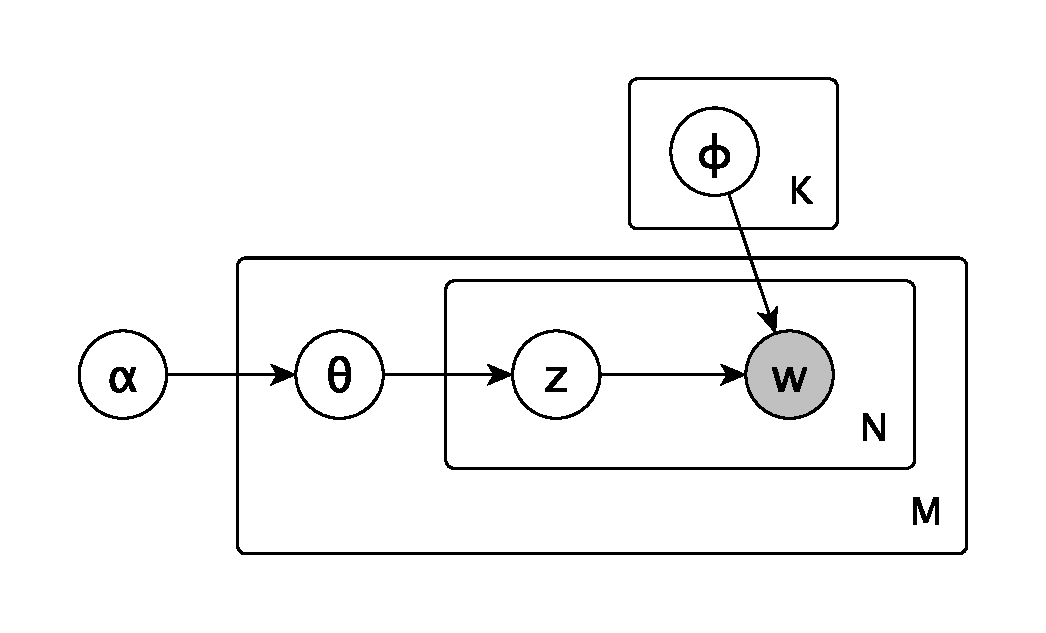
\includegraphics[scale=0.7]{figures/lda-generative-process.eps}
\caption{Diagram of the LDA model.}\label{fig:lda_gen_process}
\end{figure}

The generation of a corpus is done with the following steps~\cite{crain2012dimensionality, blei2003latent}:

\begin{itemize}
    \item \textbf{Draw a distribution over the words for each topic.}
        A sample $\Phi_i$ is drawn from a symmetric Dirichlet distribution with parameter $\beta$. 
        This sample represents the distribution of terms for the topic $i$.

        \begin{equation}
            \Phi_i \sim Dir(\beta)
        \end{equation}

        \begin{equation}
            p(\Phi_i | \beta) = \frac{\Gamma(V\beta)}{{\Gamma(\beta)}^V} \prod^V_{v=1}\phi^{\beta-1}_{iv}
        \end{equation}

        Here, $\Gamma$ is the gamma function, and $\phi_{iv}$ is the probability for a word $v$ in the topic $i$.

    \item \textbf{Draw a distribution over the topics for each document.}
        A sample $\theta_d$ is drawn from a Dirichlet distribution with parameters $\alpha$.
        This sample represents the distribution of topics for document $d$.

        \begin{equation}
            \Theta_d \sim Dir(\alpha)
        \end{equation}

        \begin{equation}
            p(\Theta_d | \alpha) = \frac{\Gamma(\sum^K_{i=1}\alpha_i)}{\prod_{i=1}^K\Gamma(\alpha_i)}\prod_{i=1}^K\theta_{di}^{\alpha_i-1}
        \end{equation}

        Here, $\theta_{di}$ is the probability of topic $i$ for document $d$.

    \item For each token with index $n$:

        \begin{itemize}
            \item \textbf{Draw a topic assignment $z_{dn}$ for the token index $n$.} 
                $z_{dn}$ is drawn from the distribution over topics for each document. 
                That is, $z_{dn}$ is drawn from a multinomial distribution using $\theta_d$ as a parameter.

                \begin{equation}
                    z_{dn} \sim Multinomial(\Theta_d)
                \end{equation}

                \begin{equation}
                    p(z_{dn} = i | \Theta_d) = \theta_{di}
                \end{equation}

            \item \textbf{Draw a token $w_{dn}$.}
                The token $w_{dn}$ is drawn from the topic distribution assigned to the index $n$.
                That is, $w_{dn}$ is drawn from a multinomial with parameter $\phi_{z_{dn}}$.

                \begin{equation}
                    w_{dn} \sim Multinomial(\Phi_{z_{dn}})
                \end{equation}

                \begin{equation}
                    p(w_{dn}=v|z_{dn}=i,\Phi_i) = \phi_{iv}
                \end{equation}

        \end{itemize}

\end{itemize}

The LDA model identifies topics from different terms that occur in the same document.
Consider the case where an LDA model has been used to learn a number of topics.
Two terms that frequently occur together are then likely to be in the same topic.
So, if the same word has been used to express different thoughts, and the word has the same probability in two topics, the words that it co-occurs with can be used to differentiate between the different thoughts.

The task of learning the LDA model is a Bayesian Inference problem.
We have several variables that we cannot observe: the word distribution for the topics ($\phi_i$), the topic assignments for the tokens ($z$), and the topic distribution for the documents ($\theta_d$).
The only observed variables are the words in the document.
We have to approximate the posterior distribution using some sampling method, since it cannot be inferred automatically~\cite{blei2003latent}.

There exist a few algorithms that can be used to learn topics for the LDA model. 
Two of these that has shown to be able to extract useful topics from text are \textit{collapsed Gibbs sampling}~\cite{griffiths2004finding} and \textit{variational Bayes}~\cite{blei2003latent}.  
Variational Bayes works by using simple single-variable models to approximate the LDA\@. 
As a consequence, it disregards any dependencies between the variables.

\subsubsection{Collapsed Gibbs Sampling}

Gibbs sampling is a Markov chain Monte Carlo (MCMC) method that is often used to obtain a good estimate for the distribution of a probability model, when it is not feasible to sample the distribution directly~\cite{crain2012dimensionality}.
With the help of a heuristic, or randomly, Gibbs sampling initializes the variables.
During a large number of iterations the variables are then sampled.
When a variable is being sampled, it is conditioned on the others.
In an MCMC fashion, a number of samples are rejected during an initial burn-in period.
This is done in order to get to a state where the points are more representative of the distribution that is estimated.

Griffith et al\@.~\cite{griffiths2004finding} came up with collapsed Gibbs sampling for the LDA model, where $\theta$ and $\phi$ are marginalized out.
The only variable to then be repeatedly sampled is the topic assignment, $z_{dn}$, conditioned on the assignments of the other tokens.

\subsection{Text Clustering}

Cluster analysis is a method to find groups in a given dataset.
The members of these groups are determined to be similar by a similarity measure~\cite{kaufman2009finding, aggarwal2012survey}.
Text data is sparse but very high dimensional.
With one dimension per term in the dictionary, it is not uncommon with dimensions in the order of $10^5$.
For this reason, some of the more naive clustering algorithms do not work well for text data~\cite{aggarwal2012survey}.

In distance-based clustering, a similarity function is used to measure the closeness between two text documents.
For the purpose of measuring the similarity between text objects, the cosine similarity function is commonly used, as well as Euclidean distance~\cite{aggarwal2012survey}.
Given two $n$ dimensional points $a$ and $b$, the definitions for the two can be seen in Equation~\ref{eq:cosine} and Equation~\ref{eq:euclidean}.
Two different approaches to distance-based clustering are distance-based partitioning and agglomerative hierarchical clustering.
For the distance-based approach, $k$-means and $k$-medoid are two frequently used algorithms.

\begin{equation}\label{eq:cosine}
    similarity(a, b) = \frac{\sum_{i=1}^n a_i b_i}{\sqrt{\sum_{i=1}^n a_i^2}\sqrt{\sum_{i=1}^n b_i^2}}
\end{equation}

\begin{equation}\label{eq:euclidean}
    d(a, b) = \sqrt{(a_1 - b_1)^2 + (a_2 - b_2)^2 + \hdots + (a_n - b_n)^2}
\end{equation}

\subsubsection{$k$-means Clustering}\label{sec:k-mean}

When using the $k$-means clustering algorithm, the clusters are based upon an initial set of $k$ representatives.
A simple approach to $k$-means clustering could look as follows:

\begin{enumerate}
    \item Select K seeds from the dataset
    \item \label{enum:k-means-step-2} Assign the rest of the documents to one of these seeds, based on how similar they are by the similarity function
    \item \label{enum:k-means-step-3} Before each new iteration, select a new centroid for each cluster. This should be the point that is the best central point for the cluster.
    \item Repeat step \ref{enum:k-means-step-2} and \ref{enum:k-means-step-3} until convergence.
\end{enumerate}

A visualization of this can be seen in Figure~\ref{fig:kmeans-iterations}.
$k$-means require a small number of iterations, an advantage it has when compared to $k$-medoid~\cite{aggarwal2012survey, schutze1997projections}.
However, $k$-means can be affected a lot by the selection of initial seeds.
One approach is to just select them randomly, or selecting them based on the result of another lightweight clustering method.
A frequently used method is $k$-means++, that has been shown to improve both the speed and accuracy of $k$-means clustering~\cite{arthur2007k}.

\begin{figure}
    \centering
    \thirdsubfig{kmeans-init}{Initial seeds}
    \thirdsubfig{kmeans-iter1}{Iteration 1}
    \quad
    \thirdsubfig{kmeans-init2}{Centroids after iteration 1}
    \thirdsubfig{kmeans-iter2}{Iteration 2}
    \thirdsubfig{kmeans-init3}{Centroids after iteration 2}
    \caption{(a) to (e) shows iterations of $k$-means until convergence.
        In (e) it can be seen that the new centroids capture the same documents as the previous iteration, and we have converged.
        The circles represents the seeds for the clusters and the data points are represented by squares.
        The color of the points are shows which cluster the point is currently assigned to.}
    \label{fig:kmeans-iterations}
\end{figure}

\subsection{Word Embeddings}

Word embeddings is the process of representing a word as a real-valued vector instead of just an atomic unit.
Viewing a word as a vector allows for doing interesting things with them, such as evaluating how similar two words are.
Evaluating the similarity of words is hard to do when treating them as atomic units.

Word embeddings can be created by using a co-occurrence matrix to see how often certain words occur together, and then perform some dimensionality reduction on them~\cite{lebret2013word, levy2014neural}.
Another approach that has been shown to be very successful in producing high-quality word embeddings is \textit{word2vec}, which uses a neural network to accomplish this task~\cite{mikolov2013efficient}.
In addition to being able to compute similarities between words, using simple algebra some interesting relationships can be discovered.
The example that Mikolav et al\@.~\cite{mikolov2013efficient} showed was that using the vector for ``King'', subtracting the vector for ``Man'' and adding the vector for ``Woman'' resulted in a vector that was close to that representing ``Queen''.

One approach to using neural networks for word embeddings is the continuous bag-of-words model~\cite{mikolov2013efficient}.
The network is used to predict a word using both words occurring both before and after it.
The words occurring before and after are used without regard to their order, which is the reason for the bag-of-words name.

The second approach that Mikolav et al\@. explored was a continuous skip-gram model~\cite{mikolov2013efficient}.
With this approach, a neural network uses the word as input. 
Based on this the network tries to predict words that co-occur with it, within a certain range.
A bigger range is more computationally complex but results in word vectors of higher quality.

Word2vec does not require labels to be provided with the data but rather uses the data itself to generate targets.
For this reason it is sometimes called a self-supervised technique.

\section{Evaluation Metrics}\label{sec:evaluation-metrics}

For classification or information retrieval systems, the typical evaluation metrics in use are \textit{precision}, \textit{recall} and \textit{recall}~\cite{jiang2012information}.
We define the following metrics in terms of \textit{true positives}, \textit{false positives}, \textit{true negatives} and \textit{false negatives}.
How they are defined can be seen in Table~\ref{tab:conf-matr}.
Data points that are correctly classified are then either \textit{true positives} or \textit{true negatives}.

\begin{table}
    \begin{center}
        \begin{tabular}{c c c}
            & Correct P & Correct N \\
            \toprule
            Predicted P & True Positive & False Positive \\
            Predicted N & False Negative & True Negative \\
        \end{tabular}
    \end{center}
    \caption{Confusion matrix for showing true positives, false positives, true negatives and false negatives}\label{tab:conf-matr}
\end{table}

Precision is the percentage of the results found by the system that are correct~\cite{tjong2003introduction}.
Recall is the percentage of correct results in the dataset that are found by the system.
Precision and recall are defined as follows:

\begin{equation}
    Precision = \frac{tp}{tp+fp}
\end{equation}

\begin{equation}
    Recall = \frac{tp}{tp+fn}
\end{equation}

F-score is the harmonic mean between recall and precision, and is defined as~\cite{tjong2003introduction}:

\begin{equation}
    F = \frac{2*precision*recall}{precision+recall}
\end{equation}

Another metric that is used for evaluation is \textit{accuracy}, which is the percentage of predictions that matches the actual labels.
Accuracy is defined as follows:

\begin{equation}
    Accuracy = \frac{tp+tn}{tp+tn+fp+fn}
\end{equation}

These metrics are designed to work when there are two labels.
Given several labels, there are different average methods used to get a score for the system.
Two of these are \textit{micro} and \textit{macro} averaging.

The number of true positives, false positives, true negatives and false negatives for the $\i$th binary classifier are here denoted as $tp_i$, $fp_i$, $tn_i$ and $fn_i$.
A binary evaluation measure on these is denoted as $B(tp_i, fp_i, tn_i, fn_i)$, e.g. $B$ could be the recall measure.
Micro-averaging works by summing the individual true positives, false positives, true negatives and false negatives~\cite{tsoumakas2009mining}.
Then you use the sums to obtain the final score.
Using the notation established above, the micro average is defined as~\cite{tsoumakas2009mining}:
\begin{equation}
    B_{micro} = B(\sum_{i = 1}^ktp_i, \sum_{i = 1}^kfp_i, \sum_{i = 1}^ktn_i, \sum_{i = 1}^kfn_i)
\end{equation}

Macro-average on the other hand works by first calculating the binary measure, and then taking the average of all of them~\cite{tsoumakas2009mining}.
It is defined as:
\begin{equation}
    B_{macro} = \frac{1}{k}\sum_{i = 1}^kB(tp_i, fp_i, tn_i, fn_i)
\end{equation}

It is worth noting that for some measures, such as Accuracy, the result of the two averaging approaches is the same.
However, it differs for \textit{recall} and \textit{precision}, and therefore also the \textit{$F_1$-score}~\cite{tsoumakas2009mining}.
The macro-average does not show skewness in the class labels since all different binary classifiers are treated equally.
If one class has a lot more cases, this is taken into account when using micro-averaging.

Perplexity can be used in order to compare different probabilistic models. 
It is a measurement that determines how good a models predictions are, where a lower score means that the model is better at predicting.
By evaluating the perplexity on a test set, it will give an indication of how well the model will generalize~\cite{blei2003latent}.
Perplexity for a set of $M$ documents, on a dataset $D$ is:
\begin{equation}
    perplexity(D) = \exp \big \{ -\frac{\sum_{i=1}^M \log p(x_i) }{M} \big \}
\end{equation}

\chapter{Method}
\label{cha:method}

The task of making a better system for labeling clinical reports was approached with different text mining techniques, support vector machines and three active learning strategies.
At first, the framework and tools used in the system are described, followed by a description of the provided dataset.
This chapter starts with describing the framework and tools used in the system and experiments.
After that there will be a description of the datasets used.
Finally, the experiments used to answer the research questions are presented.

\section{Frameworks, Tools and Implementation}
The entire system was written in Python.
The motivation behind this choice was mainly that, when it comes to machine learning and text mining, most of the existing infrastructure at Sectra is using Python.
This, in combination with the fact that there exists several tools for these purposes in Python, such as \textit{numpy} \footnote{Numpy, http://www.numpy.org/}, \textit{nltk} \footnote{Natural Language Toolkit, https://www.nltk.org/}, \textit{scikit-learn} \footnote{scikit-learn, http://scikit-learn.org/stable/} and \textit{gensim} \footnote{Gensim, https://radimrehurek.com/gensim/}.
Most of the plotting was done using the \textit{seaborn} \footnote{Seaborn, https://seaborn.pydata.org/} and \textit{bokeh} \footnote{Bokeh, https://bokeh.pydata.org/en/latest/} libraries.
\textit{pyLDAvis} \footnote{pyLDAvis, https://github.com/bmabey/pyLDAvis} was used for some additional visualization purposes with regards to topic models.

However, when it comes to active learning, there does not seem to be a proven mainstream library that contains a set of readily available algorithms.
In order to achieve better integration between the active learning system and the existing infrastructure at Sectra, as well as making adaptions such as the number of items queried in each iteration, an active learning framework was written from scratch.
The ground for this framework were the algorithms presented in Section~\ref{sec:active-learning}.

This framework consisted of three modules, called \textit{model}, \textit{dataset}, and \textit{query strategy}.
The model is a wrapper around different machine learning models.
By providing an interface for a distance or certainty measure, any underlying model able to provide such an interface can be incorporated.
For accessing the data pool a dataset wrapper was written, with an interface for accessing the labeled and unlabeled pools.
Putting this in its own module opens up the possibility for using several different storage solutions, such as a database or plain text files.
The query strategy module contains the different active learning algorithms for selecting what sample to label next.

\section{Datasets}\label{sec:datasets}

Two different datasets were used in thisthesis.
They were the dataset of clinical reports provided by Sectra, as well as Reuters-21578 \footnote{Reuters-21578, https://archive.ics.uci.edu/ml/datasets/reuters-21578+text+categorization+collection}.
The latter was used in order to be able to simulate a multi-label labeling process.
Before being integrated into Sectra's system, the different strategies needed to be evaluated from an objective point of view, so that any tradeoffs were known beforehand.
Since the vast majority of the dataset from Sectra was unlabeled, this could not effectively been done using only that.

The set of reports provided by Sectra contained 1068904 different entries, where 493 were initially labeled.
The entries were spread out over several files and stored in the JSON format.
However, those labels were subject to change, so they were mainly used to see if there was a correlation between the labels and clusters during the exploration phase.
A sample report can be seen in Figure~\ref{fig:sample-report}.
The fields include:
\begin{enumerate}
    \item \textbf{ExamId}: The ID of the exam.
    \item \textbf{ReportText}: The text for the report written by the physician after the examination.
    \item \textbf{Anamnesis}: The patient's medical history.
    \item \textbf{PatientAlert}: Anything special about the patient.
    \item \textbf{ExamComment}: Comments regarding the performed examination.
    \item \textbf{Cancelled}: Whether or not the examination was Cancelled.
    \item \textbf{ExamName}: Name of the exam.
    \item \textbf{ExamCode}: Code for the exam.
    \item \textbf{PatientSex}: The sex of the patient.
    \item \textbf{PatientAge}: Age of the patient. This field is truncated if it is above 90 years.
    \item \textbf{Urgent}: If the examination is urgent or not.
    \item \textbf{Pharma}: List of administrated pharmaceuticals.
\end{enumerate}
\begin{figure}
\begin{verbatim}
    {
        'ExamId':       3302250, 
        'ReportText':   '[NUM-SEQ] 
                        Craniell datortomografi utan och med 
                        intravenös kontrast:
                        
                        Frontalt på höger sida finns ett c:a 
                        4 x 3 cm stort lågattenuerande område, tolkas 
                        representera rest efter genomgången 
                        parenchymskada, troligen äldre kontusionsblödning. 
                        Subcorticalt på ömse sidor om centralfåran på 
                        höger sida finns ett några cm-stort 
                        lågattenuerande område som kan vara ischemiskt. 
                        Lätt sänkt attenuering av vit substans 
                        periventrikulärt förenlig med leuko-araios av 
                        degenerativ natur. För åldern normalstora 
                        ventriklar. Corticala sulci upp mot konvexiteten 
                        är något smalare än förväntat för åldern. 
                        
                        Någon tumörsuspekt förändring påvisas ej.',
        'Canceled':     False, 
        'Question':     'Förändring vä temporalt?',
        'PatientAlert': 'Hepatit C-positiv.', 
        'ExamComment':  "Alla kontrastfrågor: UA mnn", 
        'ExamName':     'DT hjärna utan och med iv kontrast',
        'Anamnesis':    'Pat med skalltrauma på 60-talet. Kommer nu med 
                        nattliga från-varoattacker. Skrikigt beteende 
                        som tolkats som epilepsi. CT är aldrig gjort. 
                        HEPATIT C-positiv."',
        'ExamCode':     '81081', 
        'PatientSex':   'MALE', 
        'PatientAge':   59, 
        'Urgent':       0, 
        'Pharma':       [{"ExamId": 3200240, "Units": "100 ml", 
                        "Pharma": "Omnipaque Inj.lösn 300 mg I/ml"}]
    }
\end{verbatim}
\caption{A sample report from the dataset provided by Sectra}
\label{fig:sample-report}
\end{figure}

The work was mainly concerned with the ReportText field, since it contains the response to the result of the examination.
But the for the complete Active Learning system the Anamnesis was used as well.
The labels that were initially assigned to these reports were:
``Blödning'', ``Infektion'', ``Metabol'', ``Tumör'', ``Cysta'', ``Missbildning'', ``Syndrom'', ``Demens'', ``Hydrocefalus'', ``Infarkt'', ``Kärlsjukdom'', ``Trauma'', ``Systemsjukdom'', ``Inklämmning'' and ``Normal''.
The distribution of categories among these initially labeled reports can be seen in Figure~\ref{fig:class-distribution}
Note that this is only a count of the different labels.
The plot is therefore is disregarding which labels occurred together.

\begin{figure}
    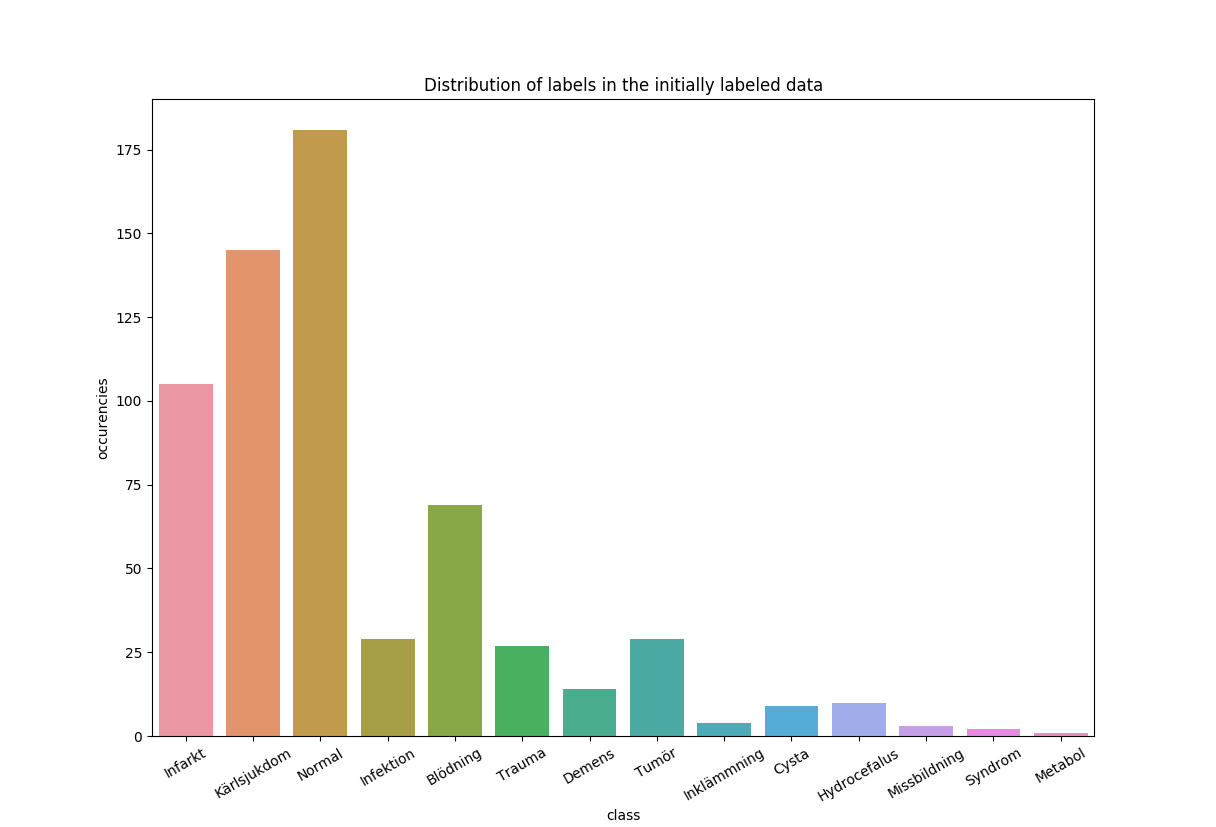
\includegraphics[scale=0.5]{figures/class-distribution.png}
    \caption{The distribution over the labels in the initial set of labeled data provided by Sectra}
    \label{fig:class-distribution}
\end{figure}

The Reuters-21578 newswire dataset is widely used when it comes to text classification research, and provides a good multi-label benchmark that can be used to compare how well certain techniques perform to other papers.
All experiments used the \textit{ModApte} split of the dataset, which is commonly used and readily available. %TODO: Footnote with the dataset?
It splits the dataset into a predefined set of training and test documents, containing 7.769 and 3.019 entries respectively.
This split contains a subset of the categories, specifically 90 different ones.
Since the clinical dataset from Sectra only contained 15 different categories, this would not mirror that very well, so instead the 15 most common categories of those were taken out.
The distribution of the top 15 Reuters-21578 categories can be seen in Figure~\ref{fig:class-distribution-reuters}.
After filtering out the documents not labeled with any of the top 15 categories, there were 6880 documents left in the training set, and 2646 in the test set.

\begin{figure}
    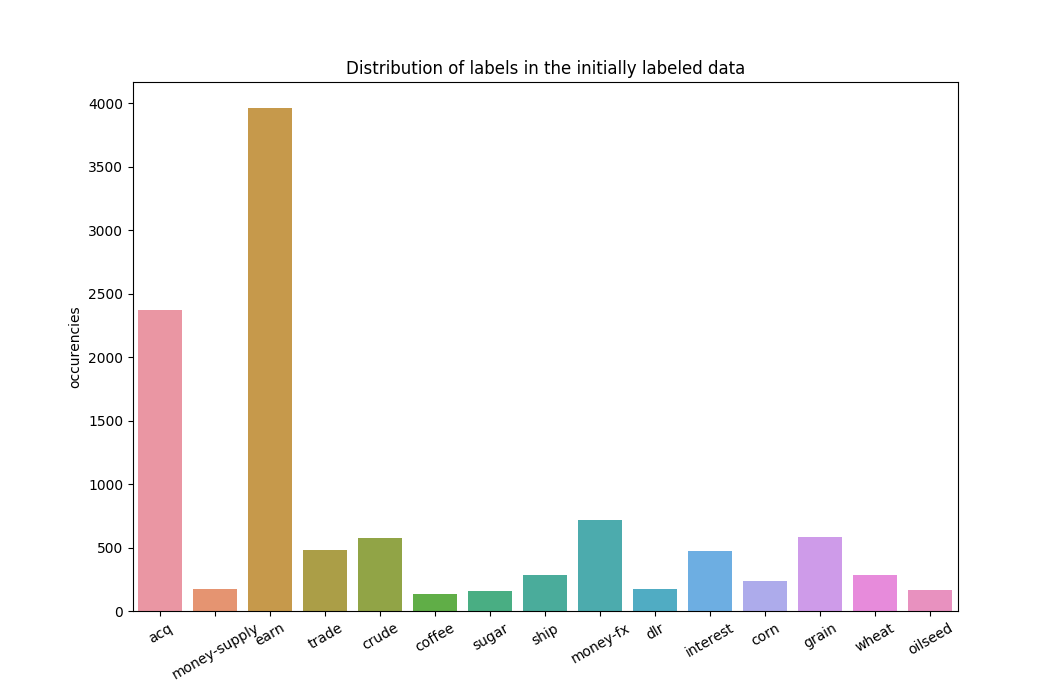
\includegraphics[scale=0.6]{figures/class-distribution-reuters.png}
    \caption{The distribution over the labels in the Reuters data}
    \label{fig:class-distribution-reuters}
\end{figure}

\section{Pre-Processing and Text Representation}\label{sec:pre-processing}

Before the data was used in the conducted experiments, several pre-processing steps were applied in order to clean the dataset and make it easier to work with.
The steps were:
\begin{enumerate}
    \item The first step was to extract the fields of interest.
          For the exploratory phase, and for the use of active learning techniques these were ``ReportText'' and ``Anamnesis''.
          When it came to filter out invalid reports, the ``ReportText'' was the only field of concern.
          It describes the results of the examination, and therefore if there was an examination at all.
    \item White space and punctuation were stripped from the data.
    \item All words were transformed into lowercase.
    \item The most common words as well as very infrequent words were both filtered out.
          Specifically, words occurring in less than 1\% of the documents, and words occurring in more than 90\% were removed.
          The idea behind this is that these words would not contribute to differentiating different classes of documents.
          Removing of both frequent and infrequent words is commonly done when working with text and has been done in the context of classification, active learning or topic modeling before~\cite{tong2001support, blei2003latent, brinker2006active, sarioglu2013topic}.
    \item A list of identified common stopwords were removed as well.
          This list of words was based on the Swedish nltk stopwords list.
          After iterating over the dataset words that occurred frequently but were not considered to be very informative for the models were identified.
          The list of stopwords was then extended to incorporate these words as dataset-specific information.
          For example, this included names of the doctors that had written the report.
          By removing names of doctors the idea is to make the system more applicable to new reports, written by other doctors.
    \item Accents from the words were removed.
    \item The text was tokenized and then stemmed using the Swedish Porter2 stemmer \footnote{Swedish Porter Stemmer, http://snowball.tartarus.org/algorithms/swedish/stemmer.html}.
\end{enumerate}
Most of these steps have been performed in previous research  dealing with text analysis in the form of classification or active learning~\cite{tong2001support, blei2003latent, brinker2006active, sarioglu2013topic}.

After transforming the text into a sequence of tokens, the final step before using it with the models was to create a representation that would be beneficial to work with.
The representation chosen was bag of words, i.e. a matrix of tokens count.
Each document is represented by the counts of each token, disregarding the order of the tokens.
In order to get some positional information into the representation additional tokens are stored. 
The additional tokens are bigrams, which are pairs of tokens (i.e. processed words).
By storing the frequency of how often such a pair occurs in the document, alongside the regular one word tokens, some positional information is retained.

\section{Exploratory Study}\label{sec:exploratory-study}
For the exploratory study we used the representation described in Section~\ref{sec:pre-processing}.
The main goal of this phase was to get to know and to better understand the dataset.
A part of this goal was to go through the fields for the different reports to see how they worked and what values could be expected.
In order to visualize the data in a 2D plot, t-distributed stochastic neighbor embedding (t-SNE) was used.
It is a dimensionality reduction technique, that is able to transform high dimensional data into two dimensions, while working to retain as much variance as possible.

The first step was to fit an LDA model to the data.
For the purpose of exploring the data, the number of topics was chosen to be a 100, with the hope of it not resulting in too granular topics that would be hard to manually analyze.
A 100 topics is what is in the middle of the range Chang et al\@.~\cite{chang2009reading} used for evaluating the interpretability of topics.
Since the purpose of this is only to explore the data, it seemed like a sufficient starting point.
The data points were plotted in a 2D plot after reducing the dimensions using t-SNE.
Each data point was colored based on some trait that the specific data point had.
For the exploratory study, the topic with the highest probability for a given data point was used to determine the color.
A plot of this can be seen in Figure~\ref{fig:lda-dist}.
Although it might be hard to interpret as a 2D plot in this report, the bokeh library allowed for the generation an interactive plot.
Hovering over each data point would show the content of the report and the topics assigned to it, making it a convenient way to explore the data and the generated topics.

\begin{figure}
    \centering
    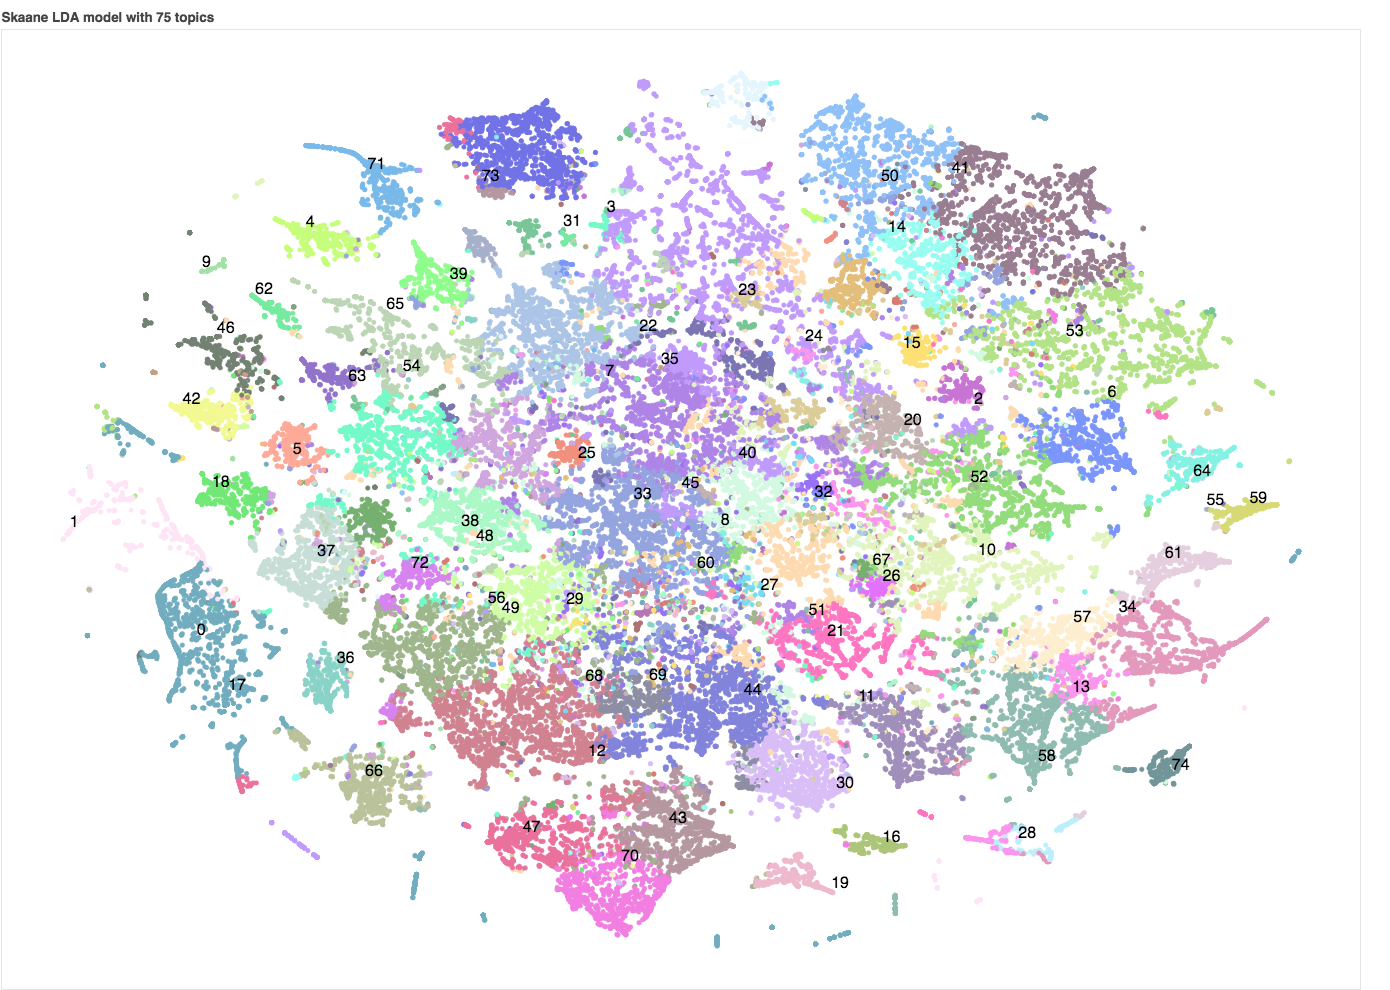
\includegraphics[scale=0.25]{figures/lda-2d-distribution.png}
    \caption{A 2D plot of the text data, where each point is colored by topic with the highest probability}
    \label{fig:lda-dist}
\end{figure}

Samples of the generated topics can be seen in Figure~\ref{fig:topic-wordclouds}.
Another way to visualize the topics for inspection is using the techniques described by Sievert et al\@.~\cite{sievert2014ldavis}.
They propose a \textit{relevance} measure where the probability for a certain term within a topic is weighted against how common that topic is in the entire corpus.
The interactive interface provided by pyLDAvis can be seen in Figure~\ref{fig:ldavis-sample}.

\begin{figure}
    \centering
    \thirdsubfigimg{wordcloud-1}{A wordcloud over the words occurring in topic 1 for an 75 topic LDA model.}
    \thirdsubfigimg{wordcloud-17}{A wordcloud over the words occurring in topic 17 for an 75 topic LDA model}
    \caption{Wordclouds for a 75 topic LDA model}
    \label{fig:topic-wordclouds}
\end{figure}

A word2vec model was used on the entire dataset to evaluate see the relationship between terms and find possible synonyms.
In order to find synonyms, all words in the dataset that had a similarity over 95\% were manually inspected.
In addition to finding synonyms, this model was used to identify names and other identifiers in the reports.
They would come up as similar entities by the model, since they are often use in the same context.
Accomplishing this was done by exploring the data through an interactive plot, after using t-SNE to reduce the number of dimensions.

\begin{figure}
    \centering
    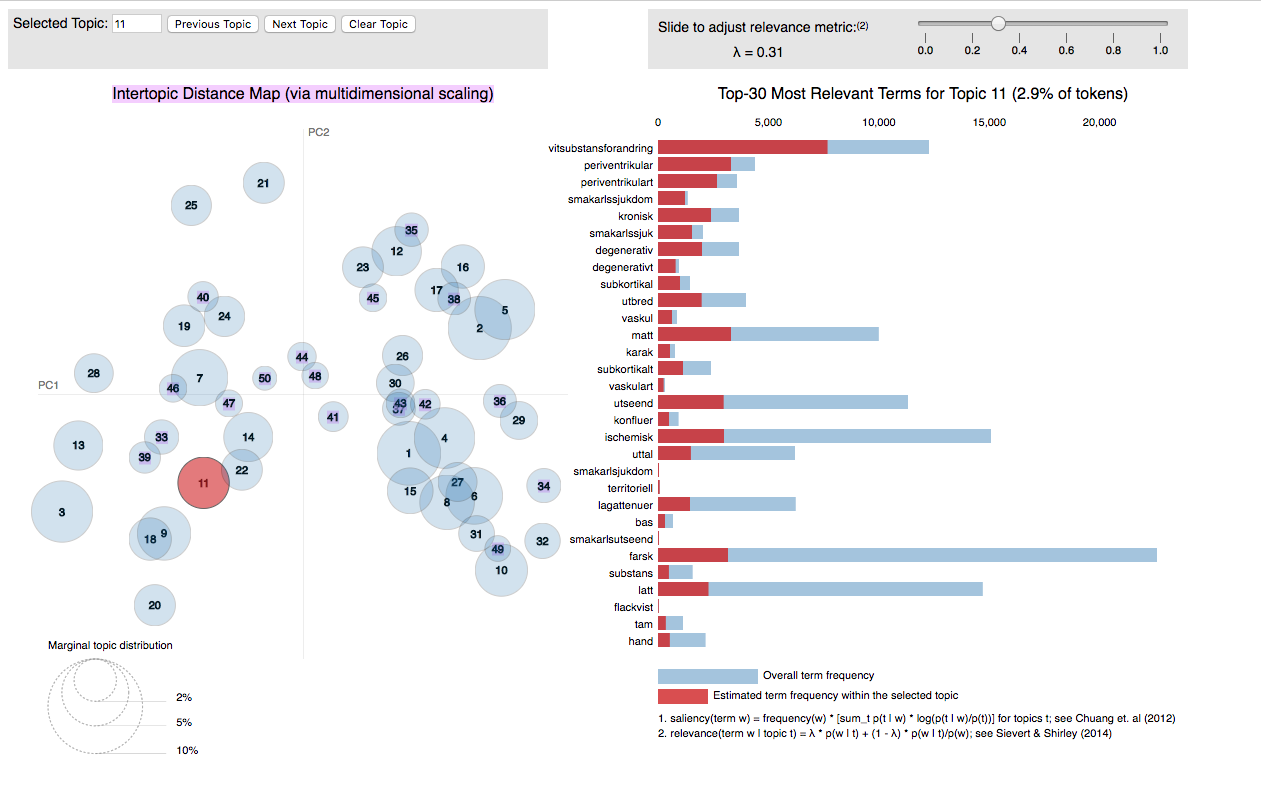
\includegraphics[scale=0.3]{figures/ldavis-sample.png}
    \caption{A way to visualize and analyze topics based on their relevance and frequency}
    \label{fig:ldavis-sample}
\end{figure}

\section{Experiments}\label{sec:exp1-method}
In this section the experiments used to answer the research questions are described.
There is one experiment designed for each question.
The first experiment is trying to identify reports that are deemed to be invalid, the second one is a study to see what the alternatives to labeling data points at random are, as well as a comparison of how well they perform according to certain metrics.
Finally, the third one aims to compare how the distribution of labels in the labeled dataset compared between the different methods.

\subsection{Filter Out Invalid Clinical Reports Using Topic Models}

The task here was to evaluate how well unsupervised techniques could be used to filter out invalid reports.
Invalid reports are considered to be reports that describe a situation where an examination never took place.
This can be because of a deceased patient, a patient being moved to another hospital, a patient did not show up or for some reason did not want to go through with the examination.

Different topic models were tested for this purpose.
The topic model used was Latent Dirichlet Allocation.
In order to use the LDA model the number of topics, $k$, has to be selected, as described in Section~\ref{sec:topic-modeling}.
The different values of $k$ that were evaluated was 25, 50, 75, 100, 150, 200.

80 000 reports were used in the experiment, and they were selected at random.
The reason for only using a subset is that the number of reports available would be too big to use in the final active learning system due to performance constraints.
The models were fitted on 72 000, or 90\%, of these reports, and the additional 10\% were used as a held-out set to evaluate the models.
To determine which topic model that should be used in the filtering of invalid reports, their perplexity was compared and the models with the lowest perplexity was chosen.
Perplexity is used in the original LDA paper by Blei et al\@.~\cite{blei2003latent} to compare different number of topics.
Hofmann used it to evaluate the pLSI based topic models as well~\cite{hofmann1999probabilistic}.

In order to evaluate how well the selected model performed on the clinical data, a set of reports had to be marked as valid/invalid.
This was done by creating a script that presented a report to the user, and requested the label.
5358 reports were labeled by the author, out of which 623 were marked as invalid. 
The labels were skewed, containing only 623 invalid reports, which makes up 10.4\% of the labels.
In order to obtain a more balanced dataset, 3653 of the valid reports were dismissed at random making it 1000 in total.
In order to make the models able to separate the invalid reports from the valid reports they had to be manually analyzed.
They are both unsupervised methods and were therefore not fitted with a specific target.
Approaching this in a way that would not result in the models overfitted to the analyzed data could potentially be hard since they are manually analyzed. 
To reduce the bias in the evaluation, the labeled reports were split into a training set and validation set, containing 80\% and 20\% of the reports respectively.
The training set was used to be analyze and identify important topics, whereas the validation set was used to evaluate how well the model performed.

First, the different topics were manually identified using the aforementioned visualization tools.
The words with the highest probability within a topic was used in order to identify topics that corresponded with terms such as cancelled or transferred.
This was done by inspecting the topics in the same way that was done in the exploratory study, Section~\ref{sec:exploratory-study}.
After that the labeled training set was used to identify more patterns among the invalid reports.
Based on the distribution of the most likely topics for the invalid reports in the training set, topics with a high indication of a report being invalid was selected for further analysis.
A combination of these topics together with the number of topics assigned with a high probability to a report were used to determine whether or not a report was invalid or not.
After some analysis, the number of topics that were assigned to a report with the probability of over 10\% was used as well.
In the report these are referred to as prominent topics.

After some initial experiments with the topics generated it was clear that the topic vectors contained patterns ripe for exploitation.
A topic vector is the vector with the topic probabilities for a document.
The patterns are clear enough to motivate the manual identification of topics that are important to differentiate between invalid and valid reports.
In order to compare this result with some more objective baseline, a logistic regression classifier was fitted on the data and evaluated as well.
A set of reports were already labeled with ``invalid'' or ``valid'' in order to evaluate the manual interpretation approach.
This set was thus used to fit the classifier.
The topic vectors were used as features, and the targets were the labels indicating if a report is valid or not.

Both of these approaches were evaluated using four different metrics, recall, precision, $F_1$-measure and accuracy.
All of which are described in Section~\ref{sec:evaluation-metrics}.

\subsection{Alternatives to Label Reports at Random}\label{sec:exp2-method}

This was done by first doing a literature study, and then exploring the relation between the initial set of labeled data with the structure of the data through clustering and topic analysis.
At first, the labeled data was transformed using the LDA and k-means models.
The k-means model used the latent topic vectors from the LDA model as representation of the text data.
After that, they were plotted in the same 2D space as before.
The color of a point in the plot was based on the first label of a sorted list of the point's labels.

Just as before this was an interactive plot, hovering over the data points revealed the report as well as the topics and the cluster assigned to the data point.
The goal of this was to see if there existed a relationship between the topics/clusters and the labeled assigned to the data point.
The relationships were explored further by creating histograms over the most likely topics for different labels, as well as histograms over categories that had a certain topic as its most likely topic.
This was done on the 4 most common labels, since most of the others lacked the amount of reports necessary to identify a clear pattern.
Even if the labels are not the same in the final system, knowledge of an existing relationship might still be exploited even if the specific labels change.
Based on multi-label nature of the data and the results of this analysis, active learning approaches were researched with the goal of identifying methods that would be applicable in a multi-label setting.
The research touched upon both methods that exploit the structure of the data, and methods that are purely uncertainty based.

After establishing the techniques that had some indication on providing a better labeling process than sampling documents at random, they were evaluated.
In the end, the algorithms described in Section~\ref{sec:active-learning} were the ones selected for evaluation.
Some motivation for the choices are presented in Chapter~\ref{cha:results}.

In order to provide a thorough evaluation of how well they techniques perform a set of already labeled documents was needed.
For this reason, the Reuters-21578 dataset was used.
The properties of the dataset, as well as a comparison between it and the clinical data provided by Sectra can be found in Section~\ref{sec:datasets}.
The dataset is common in active learning research and has been used by Brinker et al\@.~\cite{brinker2006active} and Yang et al\@.~\cite{yang2009effective}, among others.
With this set of labeled reports, a simulation of the labeling procesfs was run.
The result fot he simulation was used to compare the different strategies with regard to some evaluation metrics.
The metrics used were:
\begin{enumerate}
    \item Accuracy
    \item Micro recall
    \item Macro recall
    \item Micro precision
    \item Macro precision
    \item Micro F1-Score
    \item Macro F1-Score
\end{enumerate}

These are described in Section~\ref{sec:evaluation-metrics} and are frequently used to compare different active learning methods, for example by Yang et al\@.~\cite{yang2009effective}, Dasgupta et al\@.~\cite{dasgupta2008hierarchical} and Li et al\@.~\cite{li2013active}.

With this dataset, the same pre-processing steps that were applied to the clinical dataset were applied to the Reuters data too.
Some modifications of this includes the stopwords, instead of a curated list of words, the unmodified list of english stopwords provided by nltk was used.
The main goal was to compare how the different techniques affected the labeled dataset, and how well an SVM model performed on it.
Optimizing the process for the particular model and dataset was therefore not the focus of the study, but instead offering a more comprehensive comparison.

The strategies compared were: 
\begin{itemize}
    \item \textit{Binary Version Space Minimization}: Described in Section~\ref{subsec:binmin}
    \item \textit{Maximum Loss Reduction with Maximum Confidence}: Described in Section~\ref{subsec:mmc}
    \item \textit{Adaptive Active Learning}: Described in Section~\ref{subsec:adaptive-active-learning}
\end{itemize}
They need a small initial set of labeled reports which they can use to get initial predictions from the SVM model, upon which the strategies base their calculations.
The techniques were evaluated both by selecting this initial set of points at random, as well as selecting them from the clusters generated by the k-means algorithm.
Sampling from the clusters was done by iterating over the clusters and selecting an equal number of data points from each clusters.
All samples selected from a given cluster were chosen randomly amongst the members of the clusters.
Furthermore, the number of clusters selected was 25, in order to get an equal number of reports from each cluster in the different experimental settings.
The topic model selected in Section~\ref{sec:exp1-method} was used as input to the k-means algorithm.

Since the different models may depend on the initial samples in different ways, different initial sizes were evaluated.
This is also done by Yang et al\@.~\cite{yang2009effective}.
In their paper they tried quite large initial sample sizes.
Here, the sizes evaluated are: 25, 50, 100.
The reason for this is that an large initial sample size would make it hard for the human annotator to see a difference in the class balance early on.
The different active learning configurations that were tried is displayed in Table~\ref{fig:active-learning-configurations}
In total there were 18 configurations, based upon the three different methods.

\begin{table}
    \centering
    \begin{tabular}{|cccc|}
        \hline
        \textbf{ID} & \textbf{Active Learning Strategy} & \textbf{Initial Sampling} & \textbf{Initial Sample Size}\\
        \hline
        1 & BinMin & Random & 25\\
        2 & BinMin & Random & 50\\
        3 & BinMin & Random & 100\\
        4 & BinMin & Sampled from clusters & 25\\
        5 & BinMin & Sampled from clusters & 50\\
        6 & BinMin & Sampled from clusters & 100\\
        7 & MMC & Random & 25\\
        8 & MMC & Random & 50\\
        9 & MMC & Random & 100\\
        10 & MMC & Sampled from clusters & 25\\
        11 & MMC & Sampled from clusters & 50\\
        12 & MMC & Sampled from clusters & 100\\
        13 & Adaptive & Random & 25\\
        14 & Adaptive & Random & 50\\
        15 & Adaptive & Random & 100\\
        16 & Adaptive & Sampled from clusters & 25\\
        17 & Adaptive & Sampled from clusters & 50\\
        18 & Adaptive & Sampled from clusters & 100\\
        \hline
    \end{tabular}
    \caption{The different configurations of active learning strategies evaluated. BinMin stands for Binary Version Space Minimization, MMC stands for Maximum Loss Reduction with Maximum Confidence and Adaptive stands for Adaptive Active Learning.}
    \label{fig:active-learning-configurations}
\end{table}

\section{Evaluating the Label Balance}
The goal with the last experiment was to evaluate how the labels in the produced labeled dataset are distributed.
A set where the labels are more evenly, or uniform, distributed would be preferable.
From a perspective of the person labeling, it could feel more productive not assigning the same labels most of the time.
The more prosperous outcome from a balanced dataset would be that the models using the data in later stages could also benefit from this, and obtain better results.

The configurations used here are the same as in Table~\ref{fig:active-learning-configurations}.
Every iteration, the distribution of labels assigned are stored and analyzed.
He et al\@. discusses the usage of ROC curves and measures such as g-means to compare multi-class imbalanced data~\cite{he2009learning}.
However, the doctor involved at Sectra specifically requested that labels should be more uniformly distributed. 
The evaluation will therefore focus on measuring that instead of the models performance, which is done in ~\ref{sec:exp2-method}.
An evaluation of how the distribution progresses was done by comparing how the class imbalance is affected by the number of new samples obtained from the different methods.

Ertekin et al\@.~\cite{ertekin2007learning} used a class imbalance ratio to compare how well an active learning strategy worked.
This was only done for the binary case.
In order to get a measure for the multi-label problem, the evaluation of class imbalance was measured by the percentage of all total labels that were in the most common class, as well as in the top 3 most common classes.
Furthermore, the ratio between the biggest and the smallest class will be used in the evaluation.

\chapter{Results}
\label{cha:results}

%This chapter presents the results. Note that the results are presented
%factually, striving for objectivity as far as possible.  The results
%shall not be analyzed, discussed or evaluated.  This is left for the
%discussion chapter.

%In case the method chapter has been divided into subheadings such as
%pre-study, implementation and evaluation, the result chapter should
%have the same sub-headings. This gives a clear structure and makes the
%chapter easier to write.

%In case results are presented from a process (e.g. an implementation
%process), the main decisions made during the process must be clearly
%presented and justified. Normally, alternative attempts, etc, have
%already been described in the theory chapter, making it possible to
%refer to it as part of the justification.

In this chapter the results are described.
First, the outcome from the exploratory study is presented, followed by the different experiments.
The first experiment, filtering out invalid reports, presents the evaluation of the topic model used to filter out the reports, as well as the specific topics and how they were used in the process.
In the second one, the methods considered and the decisions behind which ones that were appropriate are presented.
Finally, the last section goes through the result of evaluating the different active learning techniques.

\section{Exploratory Study}

The goal with the exploratory study was to acquire a better understanding of the data, how it was structured and what kind of information might be extracted from it.
%[FIGURE FROM METHOD] displayed popular terms from a subset of the topics obtained from the topic model.
Certain fields such as the canceled field did not seem to be very reliable. 
Reports that clearly explained a situation where the patient had been transferred to another hospital, or for another reason not having performed an examination, still described a situation where the canceled field was set to ``false''.
After further manual analysis it was clear that the vast amount of invalid reports were contained within a few topics, something that is used in the first research question.
The evaluation of more concrete relationships were done within the context of that experiment, and is presented in Section~\ref{sec:exp1-result}.

The word2vec model produced results that allowed for synonyms to be detected.
By doing this, 420 pairs were discovered.
The vast majority of these were names and words that are used in similar contexts, which includes opposites like ``left'' and ``right''.
Some of the medical terms were hard to interpret, and were therefore not considered to be synonyms.
Disregarding these, the synonyms and misspellings that were decided to be used in the final system can be seen in Table~\ref{tab:synonyms}.
The original value was replaced with the new one during the preprocessing stage.

\begin{table}
    \centering
    \begin{tabular}{|ccc|}
        \hline
        \textbf{Original} & \textbf{Replacement} & \textbf{Type} \\
        \hline
        ordinärt & normalt & synonyms \\
        ej & inte & synonyms \\
        avbeställd & avbokad & synonyms \\
        avebställd & avbokad & misspelling + synonym \\
        belsutat & beslutat & misspelling \\
        måttliga & lätta & synonyms \\
        pat & patient & short \\
        pt & patient & short \\
        pateint & patient & misspelling \\
        akuten & akutmottagningen & misspelling \\
        us & undersökning & short \\
        \hline
    \end{tabular}
    \caption{The synonyms, misspellings and shorts found in the data that the author could assert with confidence.}
    \label{tab:synonyms}
\end{table}

In order to identify names from this word2vec model, the word vectors were plotted using the an interactive plot that allowed for exploration of the data.
Since names are commonly used in similar contexts, they have similar attributes in the word embedding model.
Figure~\ref{fig:word2vec-names-overview} shows how this was done.
Given that the names got similar coordinates in the plot, identifying the section with names allowed for identification of a lot of the names used in the reports.

\begin{figure}
    \begin{subfigure}[b]{\textwidth}
        \centering
        \fbox{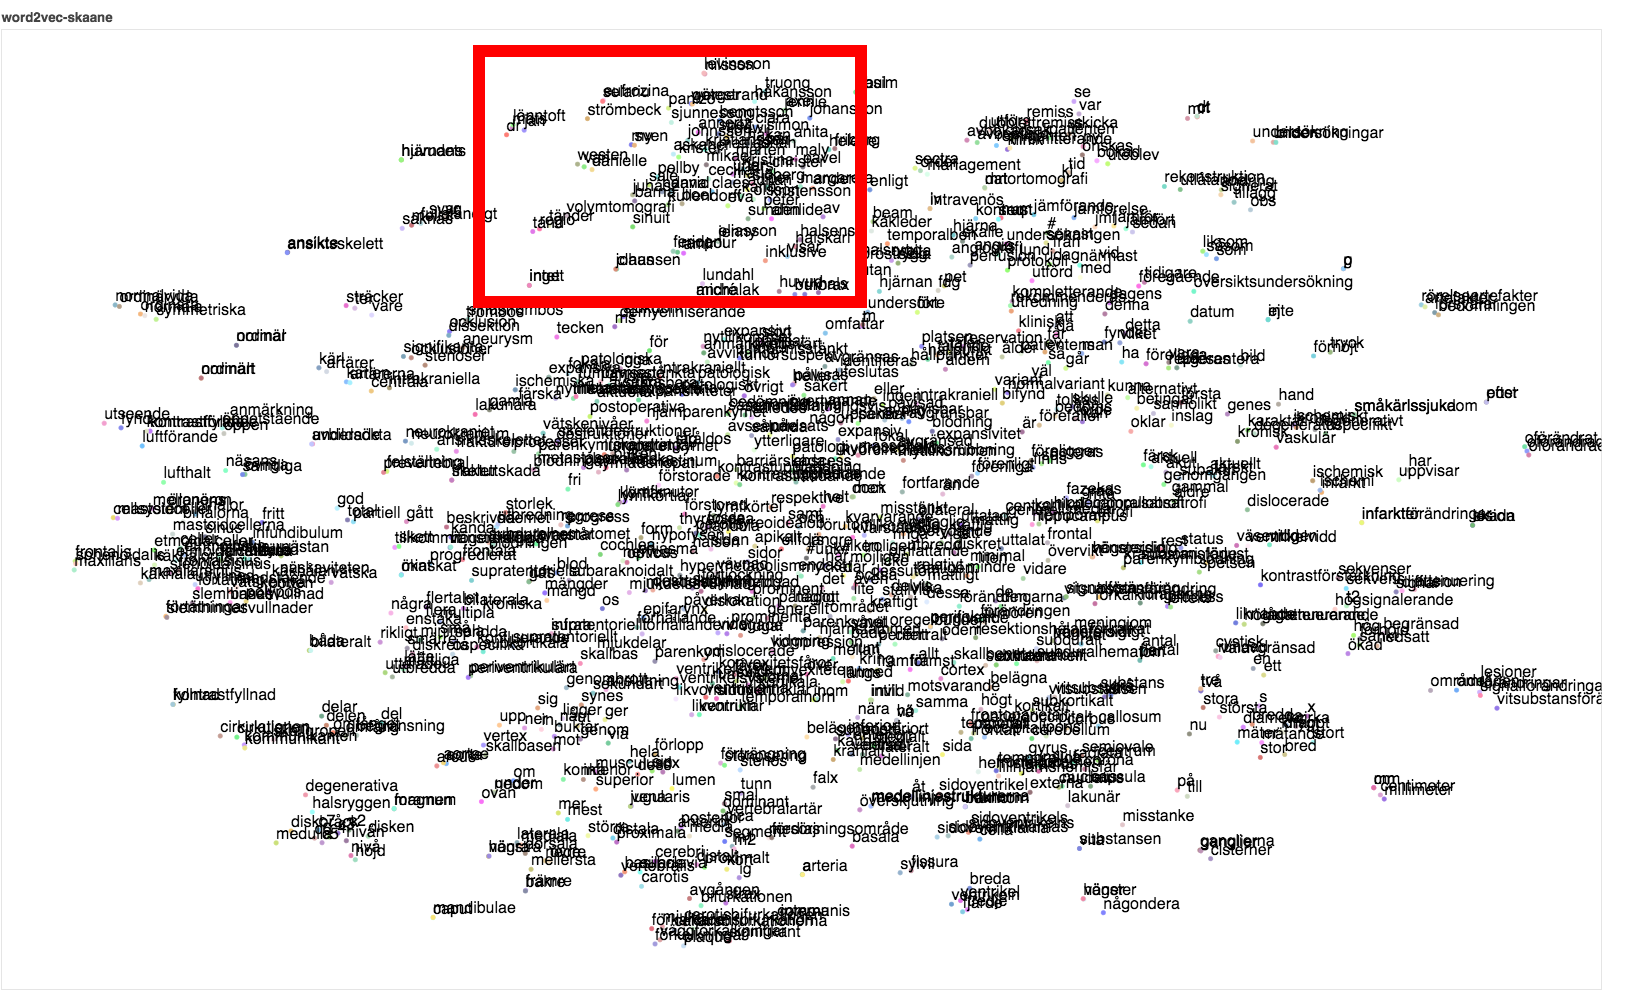
\includegraphics[width=\textwidth]{figures/word2vec-overview.png}}
        \caption{A 2D plot of the full word2vec model.}
    \end{subfigure}
    \quad
    \begin{subfigure}[b]{\textwidth}
        \centering
        \fbox{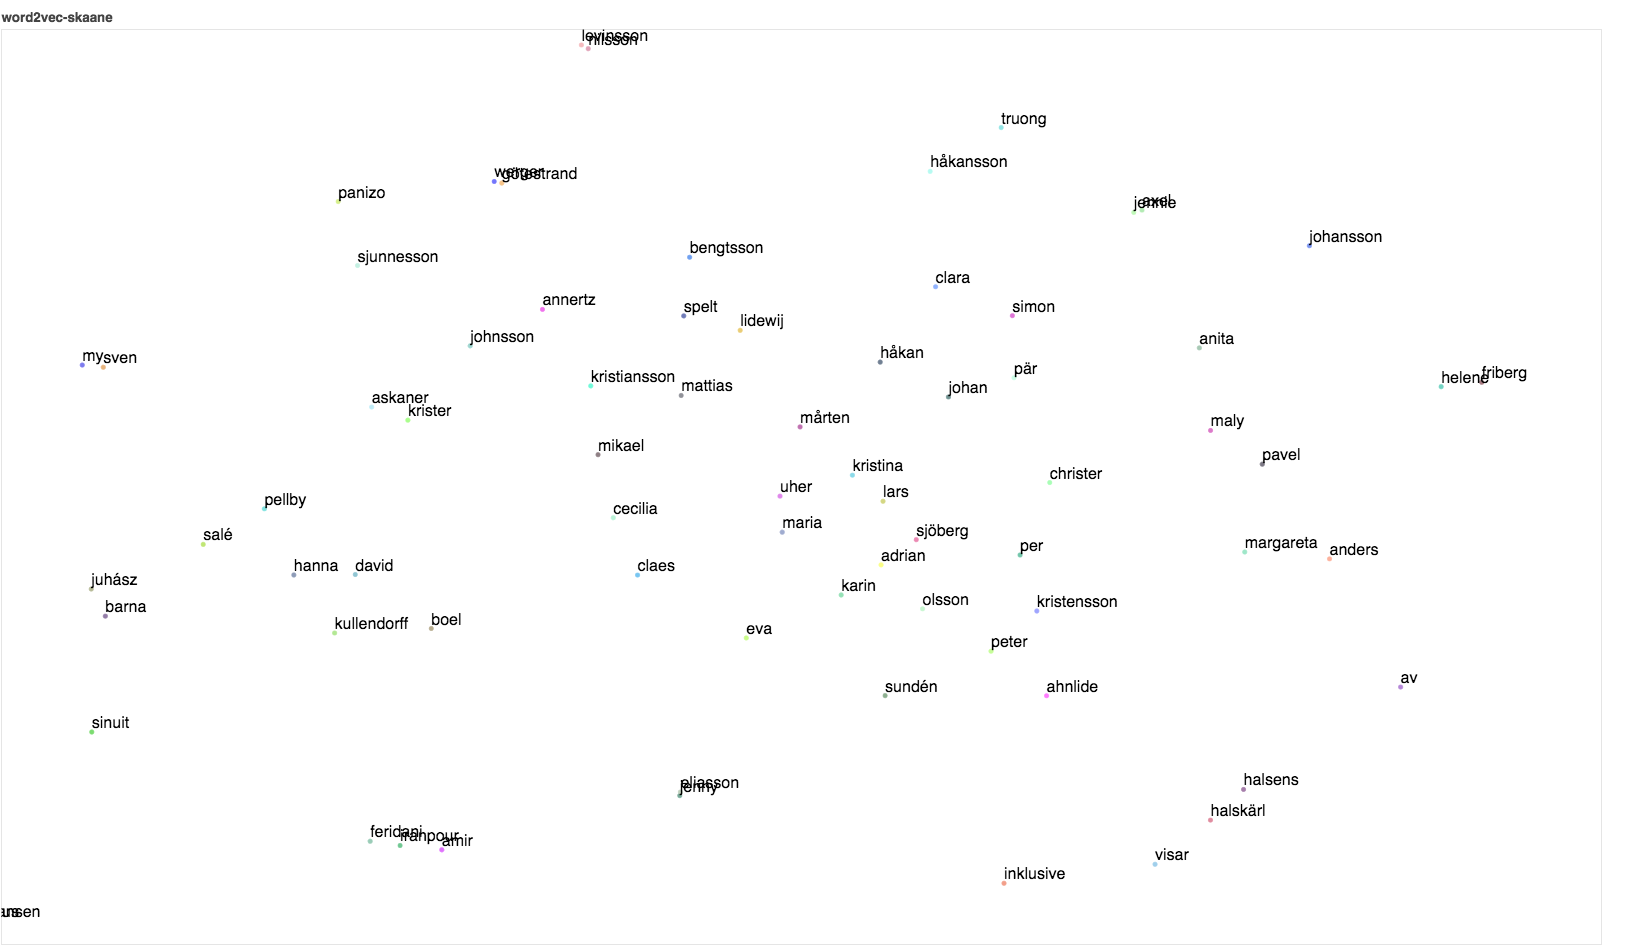
\includegraphics[width=\textwidth]{figures/word2vec-names.png}}
        \caption{A 2D plot of the subset of the word2vec model covering the names.}
    \end{subfigure}
    \caption{Two figures illustrating how the names were discovered in the word2vec plot. The (b) plot represents the red square in (a).}
    \label{fig:word2vec-names-overview}
\end{figure}

\section{Filter Out Invalid Clinical Reports Using Topic Models and Clustering}\label{sec:exp1-result}

The LDA models were evaluated by calculating the perplexity on the held-out set as described in Section~\ref{sec:exp1-method}.
Perplexity for the evaluated models can be seen in Figure~\ref{fig:lda-perplexity}, where a low score is better.
Based on this, the selected model was the LDA model with 75 topics.

\begin{figure}[h!]
    \centering
    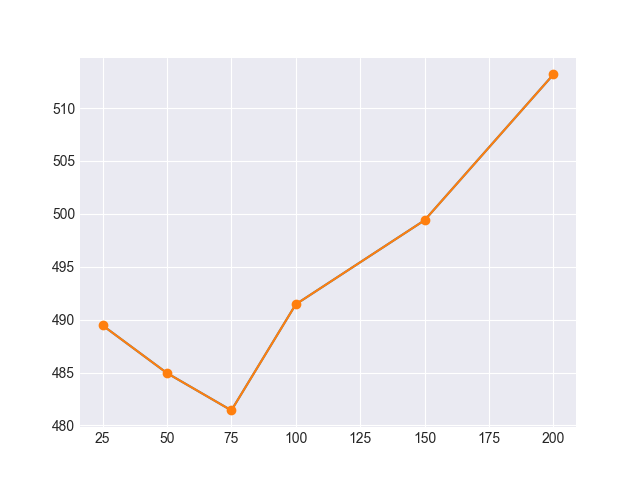
\includegraphics[width=\textwidth]{figures/lda-perplexity.png}
    \caption{The perplexity scores for the different LDA models}
    \label{fig:lda-perplexity}
\end{figure}

\begin{figure}[h!]
    \centering
    \thirdsubfigimg{invalid_reports_most_likely_topics_histogram}{The distribution of the topics with the highest probability for the invalid reports in the training set.}
    \thirdsubfigimg{valid_reports_most_likely_topics_histogram}{The distribution of the topics with the highest probability for the valid reports in the training set.}
    \caption{Distribution over the most likely topics for the valid and invalid reports. Note that only topics that occurred at least once are shown in the histogram.}
    \label{fig:most-likely-topics}
\end{figure}

The next step was identifying the topics that were assigned to the invalid reports.
First, topic 1 and 17 were identified as interesting based on the word distribution they represented.
The most common terms for these two topics can be seen in Figure~\ref{fig:topic-wordclouds}.
To verify this, the labeled data was analyzed.
The distribution of the topics with the highest likelihood for the invalid reports in the training set can be seen in Figure~\ref{fig:most-likely-topics} (a).
A couple of topics, 1 and 17 clearly stands out as the ones that most invalid reports gets assigned.
Specifically, topic 1 had a count of 131 reports from the invalid reports in the training set, and topic 17 had 358.
Some invalid reports have topics 0, 3, 9, 16, 47, 53, 58, 61, 62 as the most likely topic.
53 is the third most common, with a count of 3.

The corresponding plot for the valid reports can be seen in Figure~\ref{fig:most-likely-topics} (b).
There is a lot more variety among the most likely topics here.
Topics 1 and 17 occur very infrequently.
Topic 1 occurs 0 times, while topic 17 occurs 2 times.
The third most common topic from the invalid reports, 53, occurs 28 times.
The ones having topic 17 had 4 and 8 prominent topics assigned to them.

Each topic that was assigned to a report with a probability above 10\% was considered to be a prominent topic.
The number of prominent topics for the invalid reports can be seen in Figure~\ref{fig:prominent-topic-dist} (a).
1, 2 and 3 number of prominent topics are the most common.
And there are barely any reports having more than 6.
The corresponding plot for the valid reports can be seen in Figure~\ref{fig:prominent-topic-dist} (b).
In the case of valid reports, 6 is the most common number of prominent topics. 
The topics are a lot more spread out than in the case of the invalid reports.

\begin{figure}[h!]
    \centering
    \thirdsubfigimg{invalid_reports_prominent_topics_count_histogram}{The distribution of the number of prominent topics assigned to the invalid reports in the training set.}
    \thirdsubfigimg{valid_reports_prominent_topics_count_histogram}{The distribution of the number of prominent topics assigned to the valid reports in the training set.}
    \caption{The distribution of the number of prominent topics for the two categories.}
    \label{fig:prominent-topic-dist}
\end{figure}

Another idea was to evaluate whether or not 17 and 1 were among the most probable topics for the reports.
A simple evaluation of this on the set of valid reports showed that it was not a good approach.
For example, seeing if 17 or 1 had more than 10\% probability returned 48 and 45 valid reports, respectively.
Checking if both were above the threshold returned 11 reports.

Based on these findings, reports were determined to be invalid or not based on if they fulfilled both of the following criteria:
\begin{itemize}
    \item Having either topic 1 or 17 as its most probable topic.
    \item Not having more than 6 prominent topics assigned to it.
\end{itemize}

The evaluation on the validation set can be seen in Table~\ref{tab:exp1-eval}.
In the figure you can also see the results of the logistic regression classifier, which was fitted with the topic vectors as features and the invalid/valid labels as targets.

\begin{table}[h!]
    \centering
    \begin{tabular}{|c|cc|}
        \hline
        & \textbf{Manual Identification} & \textbf{Logistic Regression} \\
        \hline
        \textbf{Precision} & 97.2\% & 98.7\% \\
        \textbf{Recall} & 100\% & 100\% \\
        \textbf{$F_1$-measure} & 98.6\% & 99.4\%\\
        \textbf{Accuracy} & 97.9\% & 99.1\%\\
        \hline
    \end{tabular}
    \caption{The results of the classification of the invalid reports. The manual identification column represents the use of manual interpretation of the LDA topics to find the invalid reports.}
    \label{tab:exp1-eval}
\end{table}

A comparison of how long time it took for the different strategies can be seen in Figure~\ref{fig:al-time-dist}.

\begin{figure}[!ht]
    \centering
    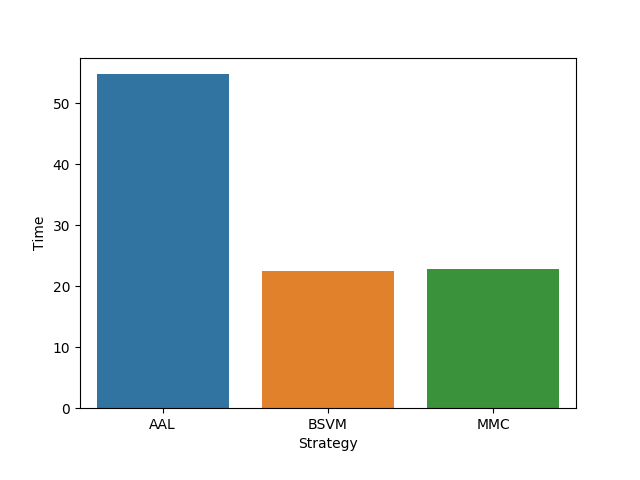
\includegraphics[width=\textwidth]{figures/time-distribution.png}
    \caption{The percentage of time used on the different strategies during one iteration.}
    \label{fig:al-time-dist}
\end{figure}

\section{Alternatives to Labeling at Random}

The first thing that was done with regards to this experiment was to explore and try to find a relationship between the initial set of labels and the inherit structure of the data.
This was done by visualizing the LDA model again.
In order to find any existing relationship between the topics and the labeled samples, the points were colored based on their assigned labels.
Unlabeled samples were hidden from the plot.
The resulting plot can be seen in Figure~\ref{fig:categories-lda-75}.
From this plot it is clear that there is a grouping of labels.
Certain labels are more likely to occur in documents assigned a specific topic.
For example, the purple points in the lower part of the graph represents the ``blödning'' label, the gray labels in the middle represents ``infarkt'' and the light blue ones that are mostly concentrated in the bottom right corner represents ``infektion''.
It is clear that these labels are not evenly spread out over all the topics, but neither are they confined enough to make a mapping between topics and labels, like they were in Section~\ref{sec:exp1-result}.

\begin{figure}[ht!]
    \centering
    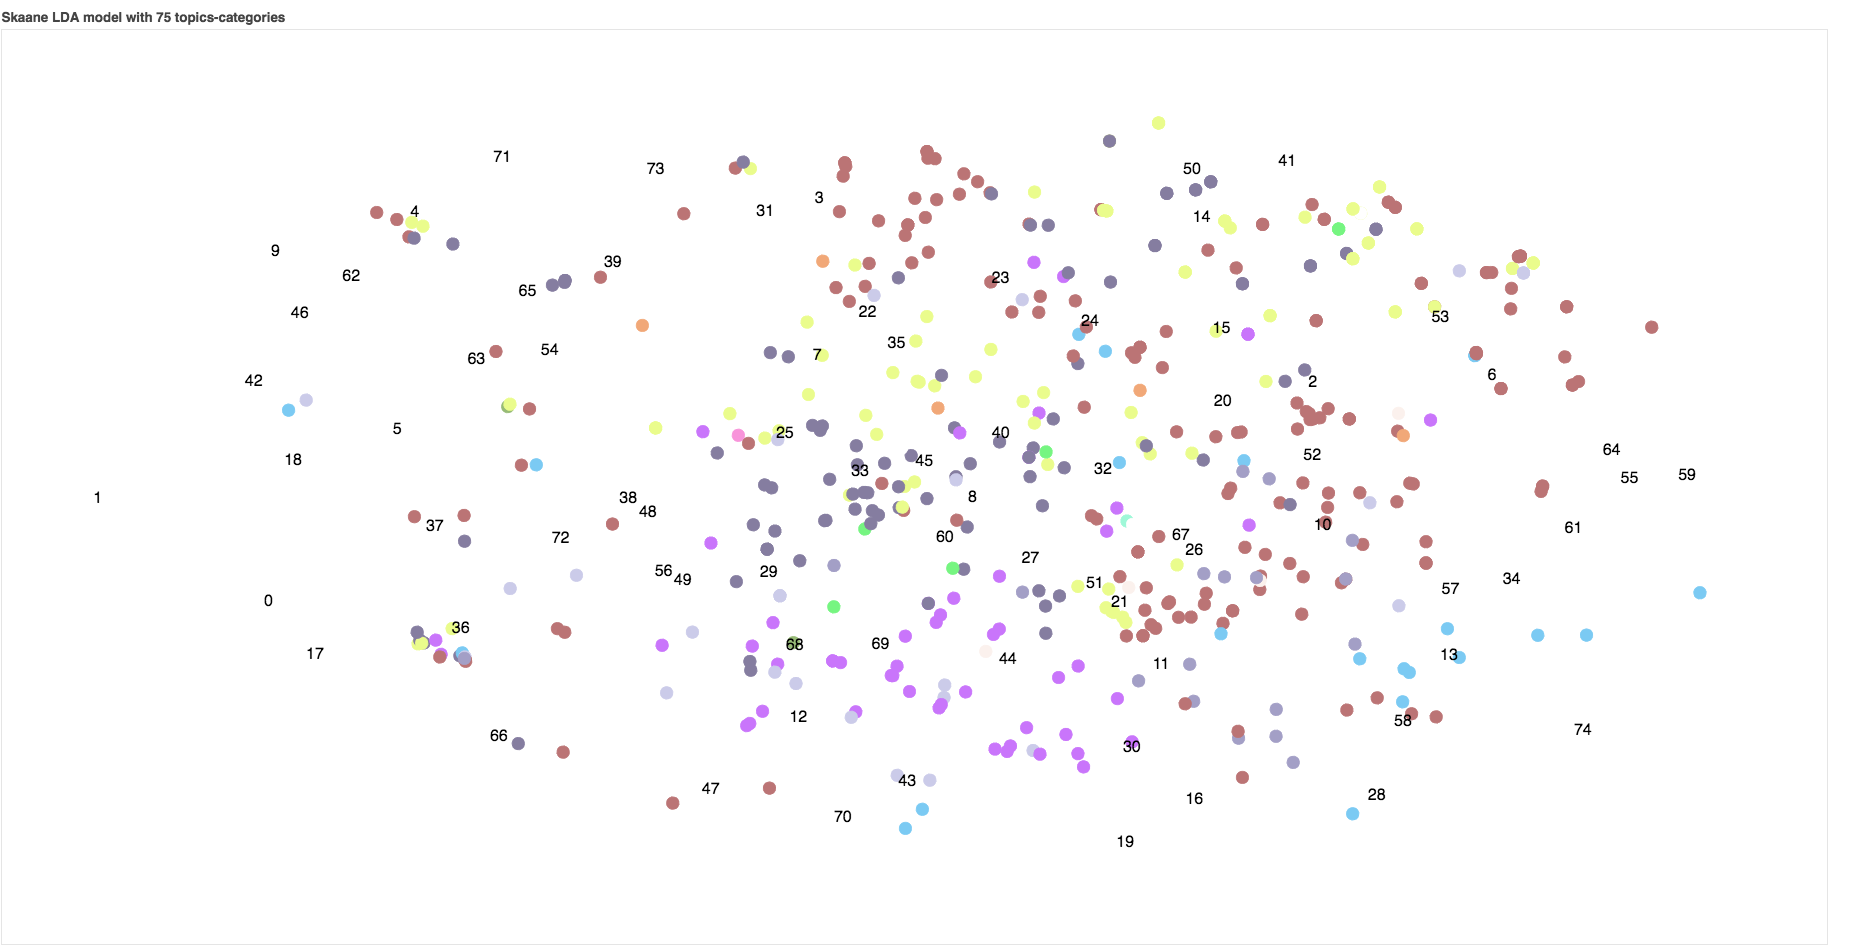
\includegraphics[width=\textwidth]{figures/categories-lda-75.png}
    \caption{The labeled data points plotted in 2D, and colored based on the first label of the report in alphabetical order.}
    \label{fig:categories-lda-75}
\end{figure}

In Figure~\ref{fig:category-label-distribution} the counts of most likely topics for the four most common categories are displayed.
These categories are ``infarkt'', ``kärlsjukdom'', ``normal'' and ``blödning''.
From the histograms it is clear that documents of a certain category are more likely to be assigned certain topics, at least in these cases.
Even though there exist a clear relationship, it is not exclusive enough to make any clear relation.
The number of topics assigned and reports labeled for these 4 topics can be seen in Table~\ref{tab:topic-categories}.

\begin{table}[ht!]
    \centering
    \begin{tabular}{|c|cc|}
        \hline
        \textbf{Label} & \textbf{No. reports} & \textbf{No. most likely topics} \\
        \hline
        Normal & 181 & 28\\
        Tumör & 29 & 15\\
        Infarkt & 105 & 27\\
        Blödning & 69 & 19\\
        Kärlsjukdom & 145 & 28\\
        Hydrocefalus & 10 & 5\\
        Demens & 14 & 9\\
        Trauma & 27 & 12\\
        Cysta & 9 & 7\\
        Missbildning & 3 & 3\\
        Inklämmning & 4 & 1\\
        Infektion & 29 & 15\\
        Syndrom & 2 & 2\\
        Metabol & 1 & 1\\
        \hline
    \end{tabular}
    \caption{The number of reports assigned a certain category, as well as the number of different topics assigned as the most likely one for reports with the given category.}
    \label{tab:topic-categories}
\end{table}

\begin{figure}[h!]
    \centering
    \thirdsubfigimg{infarkt}{The counts of most likely topics for the ``infarkt'' label.}
    \thirdsubfigimg{karlsjukdom}{The counts of most likely topics for the ``kärlsjukdom'' label.}
    \quad
    \thirdsubfigimg{normal}{The counts of most likely topics for the ``normal'' label.}
    \thirdsubfigimg{blodning}{The counts of most likely topics for the ``blödning'' label.}
    \caption{The counts of the most likely topics for the four most common categories.}
    \label{fig:category-label-distribution}
\end{figure}

In order to analyze these topics further, Figure~\ref{fig:topic-category-distribution} shows the different categories that has a certain topic assigned to it as the most likely one.
Taking into account the information from Table~\ref{tab:topic-categories}, i.e. that some categories are a lot more common than others in the labeled dataset, there is not a clear enough pattern to distinguish between different categories based on the topics.
This does not take the multi-label nature of the data into account.
If a report has multiple labels assigned to it, both of the labels are counted separately.

\begin{figure}[h!]
    \centering
    \thirdsubfigimg{categories-topic-13}{The counts categories where the most likely topic for the report was 13.}
    \thirdsubfigimg{categories-topic-16}{The counts categories where the most likely topic for the report was 16.}
    \quad
    \thirdsubfigimg{categories-topic-25}{The counts categories where the most likely topic for the report was 25.}
    \thirdsubfigimg{categories-topic-35}{The counts categories where the most likely topic for the report was 35.}
    \caption{The categories of the different reports that are assigned a certain topic as the most likely one.}
    \label{fig:topic-category-distribution}
\end{figure}

Based on the knowledge that there exists a pattern, the initial goal was to find some methods that could exploit this.
Some active learning approaches using different forms of clustering, such as Dasgupta et al\@'s approach using hierarchical clustering~\cite{dasgupta2008hierarchical}, would be good contenders.
However, the method described by Dasgupta et al\@. is made for the single-label case with no obvious way of extending the technique into multi-label.
The same applies to the density based technique suggested by Attenberg et al\@.~\cite{attenberg2013class}.

Most of the active learning research seems to be focused on binary, and maybe multi-class classification.
Thus the methods described in Section~\ref{sec:active-learning} where the ones decided on.
Methods that are fully reliant on a models certainty, such as Binary Version Space Minimization (BSVM)~\cite{brinker2006active} are used.
Furthermore, methods incorporating some information about the data in the form of label cardinality is included as well.
These techniques are Maximum Loss Reduction with Maximum Confidence (MMC) and Adaptive Active Learning (AAL)~\cite{yang2009effective, li2013active}.
An attempt to take advantage of the structure of the data is done by selecting the initial samples from different clusters, as described in Section~\ref{sec:exp2-method}.

The plot for evaluating accuracy on the strategies with initial sample sizes of 25, 50 and 100 can be seen in Figure~\ref{fig:al-accuracy-25}, Figure~\ref{fig:al-accuracy-50}, and Figure~\ref{fig:al-accuracy-100} respectively.
Note that when retrieving the initial sample from the clusters, only samples with label cardinality 1 was retrieved after 10 tries.
MMC requires at least two different label cardinalities in the initial sample in order for the logistic regression model to work.
For that reason, MMC with cluster initialization was not evaluated.
In Table~\ref{tab:active-learning-accuracy-25} to Table~\ref{tab:active-learning-accuracy-100} it can be seen how many labels were required to reach a certain accuracy.

\includeaccuracyplot{25}
\includeaccuracyplot{50}
\includeaccuracyplot{100}

\begin{table}
    \centering
    \begin{tabular}{|cccccccc|}
        \hline
        \textbf{Strategy} & \textbf{Initial Sample} & \textbf{75 \%} & \textbf{80 \%} & \textbf{85 \%} & \textbf{87 \%} & \textbf{88 \%} & \textbf{89 \%}\\
        \hline
        BSVM & Random & 475 & 650 & 1100 & 1450 & 1675 & 2425\\
        BSVM & Cluster & 425 & 650 & 1100 & 1575 & 1700 & 2425\\
        MMC & Random & 600 & 775 & 1050 & 1250 & 1575 & N/A\\
        MMC & Cluster & N/A & N/A & N/A & N/A & N/A & N/A\\
        Adaptive & Random & 400 & 575 & 975 & 2425 & N/A & N/A\\
        Adaptive & Cluster & 375 & 550 & 1025 & 2300 & N/A & N/A\\
        Random & Random & 550 & 900 & 1700 & N/A & N/A & N/A\\
        \hline
    \end{tabular}
    \caption{The number of labeled reports in total that the strategies required to achieve the different accuracy values, with initial sample size 25. Only results for the first 2500 data points that were labeled are considered.}
    \label{tab:active-learning-accuracy-25}
\end{table}

\begin{table}
    \centering
    \begin{tabular}{|cccccccc|}
        \hline
        \textbf{Strategy} & \textbf{Initial Sample} & \textbf{75 \%} & \textbf{80 \%} & \textbf{85 \%} & \textbf{87 \%} & \textbf{88 \%} & \textbf{89 \%}\\
        \hline
        BSVM & Random & 450 & 625 & 1075 & 1550 & 1750 & N/A\\
        BSVM & Cluster & 450 & 675 & 1125 & 1600 & 1725 & 2450\\
        MMC & Random & 625 & 775 & 1100 & 1325 & 1675 & N/A\\
        MMC & Cluster & N/A & N/A & N/A & N/A & N/A & N/A\\
        AAL & Random & 375 & 575 & 925 & N/A & N/A & N/A\\
        AAL & Cluster & 425 & 575 & 1075 & N/A & N/A & N/A\\
        Random & Random & 550 & 775 & 1575 & N/A & N/A & N/A\\
        \hline
    \end{tabular}
    \caption{The number of labeled reports in total that the strategies required to achieve the different accuracy values, with initial sample size 50. Only results for the first 2500 data points that were labeled are considered.}
    \label{tab:active-learning-accuracy-50}
\end{table}

\begin{table}
    \centering
    \begin{tabular}{|cccccccc|}
        \hline
        \textbf{Strategy} & \textbf{Initial Sample} & \textbf{75 \%} & \textbf{80 \%} & \textbf{85 \%} & \textbf{87 \%} & \textbf{88 \%} & \textbf{89 \%}\\
        \hline
        BSVM & Random & 400 & 600 & 1125 & 1525 & 1775 & N/A\\
        BSVM & Cluster & 450 & 675 & 1125 & 1600 & 1725 & 2450\\
        MMC & Random & 600 & 750 & 1100 & 1325 & 1675 & N/A\\
        MMC & Cluster & N/A & N/A & N/A & N/A & N/A & N/A\\
        AAL & Random & 350 & 525 & 925 & 2450 & N/A & N/A\\
        AAL & Cluster & 450 & 600 & 1025 & N/A & N/A & N/A\\
        Random & Random & 475 & 775 & 1700 & N/A & N/A & N/A\\
        \hline
    \end{tabular}
    \caption{The number of labeled reports in total that the strategies required to achieve the different accuracy values, with initial sample size 100. Only results for the first 2500 data points that were labeled are considered.}
    \label{tab:active-learning-accuracy-100}
\end{table}

The micro and macro $F_1$-score, recall and precision for the initial sample size of 25 can be seen in Figure~\ref{fig:result-25}.
The same evaluation for the initial sample size of 50 and 100 can be seen in Figure~\ref{fig:result-50} and Figure~\ref{fig:result-100}, respectively.

\includeevaluationplot{25}
\includeevaluationplot{50}
\includeevaluationplot{100}

\section{Evaluating the Label Balance}

The last part to evaluate is how the different Active Learning techniques effected the balance of the labels.
For the Reuters dataset, how the overall distribution of the labels is can be seen in Figure~\ref{fig:class-distribution-reuters}.
After random sampling, the distribution can be seen in Figure~\ref{fig:class-distribution-reuters-random}.
For comparison with the techniques it shows the labels both after 500 labels are added, and 2000.
In order to be able to compare it with the other techniques easily, the plot contains the distribution after both 500 and 2000 labels are acquired.
The distribution after sampling with the original BSVM can be seen in Figure~\ref{fig:class-distribution-reuters-binmin}, and with the initial samples taken from clusters in Figure~\ref{fig:class-distribution-reuters-binmin-clusters}.
For MMC the distribution can be seen in Figure~\ref{fig:class-distribution-reuters-mmc}.
The corresponding plots for Adaptive Active Learning can be seen in Figure~\ref{fig:class-distribution-reuters-adaptive} and Figure~\ref{fig:class-distribution-reuters-adaptive-clusters}.

\begin{figure}
    \centering
    \thirdsubfigimg{distribution-RandomSampling-25-500}{The class distribution from random sampling after 500 labels}
    \thirdsubfigimg{distribution-RandomSampling-25-2000}{The class distribution from random sampling after 2000 labels}
    \caption{The distribution of labels after random sampling}
    \label{fig:class-distribution-reuters-random}
\end{figure}

\begin{figure}
    \centering
    \thirdsubfigimg{distribution-BinaryMinimization-25-500}{The class distribution from BSVM after 500 labels}
    \thirdsubfigimg{distribution-BinaryMinimization-25-2000}{The class distribution from BSVM after 2000 labels}
    \caption{The distribution of labels after BSVM}
    \label{fig:class-distribution-reuters-binmin}
\end{figure}


\begin{figure}
    \centering
    \thirdsubfigimg{distribution-ClusterBinaryMinimization-25-500}{The class distribution from BSVM, with the initial sample from clusters, after 500 labels}
    \thirdsubfigimg{distribution-ClusterBinaryMinimization-25-2000}{The class distribution from BSVM, with the initial sample from clusters, after 2000 labels}
    \caption{The distribution of labels after BSVM with clustering}
    \label{fig:class-distribution-reuters-binmin-clusters}
\end{figure}

\begin{figure}
    \centering
    \thirdsubfigimg{distribution-MMC-25-500}{The class distribution from MMC after 500 labels}
    \thirdsubfigimg{distribution-MMC-25-2000}{The class distribution from MMC after 2000 labels}
    \caption{The distribution of labels after MMC}
    \label{fig:class-distribution-reuters-mmc}
\end{figure}

\begin{figure}
    \centering
    \thirdsubfigimg{distribution-AdaptiveLearner-25-500}{The class distribution from Adaptive Active Learning after 500 labels}
    \thirdsubfigimg{distribution-AdaptiveLearner-25-2000}{The class distribution from Adaptive Active Learning after 2000 labels}
    \caption{The distribution of labels after Adaptive Active Learning}
    \label{fig:class-distribution-reuters-adaptive}
\end{figure}

\begin{figure}
    \centering
    \thirdsubfigimg{distribution-ClusterAdaptiveLearner-25-500}{The class distribution from Adaptive Active Learning, with the initial sample from clusters, after 500 labels}
    \thirdsubfigimg{distribution-ClusterAdaptiveLearner-25-2000}{The class distribution from Adaptive Active Learning, with the initial sample from clusters, after 2000 labels}
    \caption{The distribution of labels after Adaptive Active Learning with clustering}
    \label{fig:class-distribution-reuters-adaptive-clusters}
\end{figure}

In Table~\ref{tab:distribution-result-500} the results of the evaluation after 500 new labels can be seen.
The corresponding table for the evaluation after 2000 new labels can be seen in Table~\ref{tab:distribution-result-2000}.

\begin{table}[h!]
    \centering
    \begin{tabular}{|ccccc|}
        \hline
        \textbf{Strategy} & \textbf{Initial Sample} & \textbf{Top Class} & \textbf{Top 3 Classes} & \textbf{Small/Big Ratio}\\
        \hline
        Random & Random &  34.9 \% & 65.5 \% & 32.0 \\
        BSVM & Random &  22.0 \% & 49.8 \% & 45.0 \\
        BSVM & Clusters & 19.8 \% & 49.0 \% & 80.0 \\
        Adaptive & Random & 14.8 \% & 38.5 \% & 5.4 \\
        Adaptive & Clusters & 14.5 \% & 38.2 \% & 6.65 \\
        MMC & Random & 13.1 \% & 35.2 \% & 8.2 \\
        \hline
    \end{tabular}
    \caption{The results after analyzing the label distribution after 500 new labels has been added.}
    \label{tab:distribution-result-500}
\end{table}

\begin{table}[h!]
    \centering
    \begin{tabular}{|ccccc|}
        \hline
        \textbf{Strategy} & \textbf{Initial Sample} & \textbf{Top Class} & \textbf{Top 3 Classes} & \textbf{Small/Big Ratio}\\
        \hline
        Random & Random & 36.65 \% & 64.6 \% & 29.4 \\
        BSVM & Random & 16.0 \% & 42.4 \% & 7.5 \\
        BSVM & Clusters & 15.7 \% & 41.5 \% & 7.3 \\
        Adaptive & Random & 36.4 \% & 56.2 \% & 43.4 \\
        Adaptive & Clusters & 34.5 \% & 54.8 \% & 41.0 \\
        MMC & Random & 16.7 \% & 41.2 \% & 9.3 \\
        \hline
    \end{tabular}
    \caption{The results after analyzing the label distribution after 2000 labels has been added.}
    \label{tab:distribution-result-2000}
\end{table}
\chapter{Discussion}
\label{cha:discussion}

The discussion chapter is separated into three parts.
First, it goes through and analyzes the results from Chapter~\ref{cha:results}.
This is followed by an analysis of the methods described in Chapter~\ref{cha:method}.
At last the work is discussed in a wider concept, based on the ethical and societal impact techniques like these may have.

\section{Results}
\label{sec:discussion-results}

Obtaining 97.9 \% and 99.1 \% accuracy for classifying invalid reports must be considered a good results.
The reports describing the cases where an examination did not happen uses a fairly different vocabulary.
For these cases there is a lack of medical terms, while expressions such as ``cancelled'', or ``new time'' are a lot more common.
This distinction makes it rather easy for the topic model to identify the topics relating to this.
The vocabulary is quite unique.
There is some overlap of course, the manual identification of topics did get a worse precision.
That is, it got more false misclassifications than the logistic regression model.
A probable reason for this is that there exists some information in the topics other than topic 1 and 17 that can help in identifying reports that have these as their most likely topic, but still is not invalid.
One such thing could be a more finely tuned notion of prominent topics.
However, given the clear relationship between certain topics and whether the reports are invalid, it might even be sufficient to have a finely tuned list of keywords to look for when classifying the reports.

Looking at how the different strategies perform in terms of accuracy and $F_1$-score, it is clear that for the first 600-700 labels, MMC performs considerably worse than the rest.
That is including random sampling.
It is equally clear that it performs better when the initial sample is bigger.
One reason behind this may be MMC's dependence on the label cardinality of the samples.
MMC's dependence on label cardinality can be seen in Section~\ref{subsec:mmc}.
If the information on label cardinality is not varied, the predictions that MMC base the calculations upon wont be as good.
In the paper by Yang et al\@.~\cite{yang2009effective}, MMC performs significantly better than than Binary Version Space Minimization at all stages.
One obvious reason for this discrepancy could be the implementation used in this paper, as is discussed in Section~\ref{sec:discussion-results}.
Another one can be the initial sample size used in that paper, even when they compare different initial sample sizes, they start at 100 samples and go up to a 1000.

Adaptive Active Learning performs the best of the evaluated strategies in both accuracy and $F_1$-score. 
A probable reason for this is the extra computations the strategy does in order to find the best weight between the certainty based, and the cardinality based, strategies.
Even if the cardinality predictions is not deemed to be very good in the beginning, for example, it would simply put more weight on the certainty measure.

Binary Version Space Minimization on the other hand performs very similarly to random sampling for the first samples.
The reason for this is rather simple.
In the strategy finds the class that is the closest for each data point, and selects the minimum of those.
If there are several with the same minimum value they are selected at random from those.
Until all classes has been sampled at least one, the minimum for all data points will be that class, and it will be equal among all data points.
Therefore, it will be the same as selecting randomly among all the samples, in the same way that random sampling is doing.
However, when all samples have been sampled, and quickly outperforms the random sampling in terms of accuracy and $F_1$-score.

In the end, the different strategies all perform better than random sampling.
The ones that are based on MMC and Binary Version Space Minimization tend to perform a bit better than Adaptive Active Learning when more than 1200-1300 samples are added.
This may very well be related to the fact that the distributions for MMC and Binary Version Space Minimization is considerably more uniform when a lot of labels have been requested.

Add some things regarding the initial clustering. Maybe move to earlier to have a good continuation into discussing distributions.
%Are there anything in the results that stand out and need be
%analyzed and commented on? 

% How do the results relate to the
%material covered in the theory chapter? What does the theory
%imply about the meaning of the results? For example, what
%does it mean that a certain system got a certain numeric value
%in a usability evaluation; how good or bad is it? Is there
%something in the results that is unexpected based on the
%literature review, or is everything as one would theoretically
%expect?

\section{Method}
\label{sec:discussion-method}

Results that are based on a public dataset are naturally easier to reproduce.
The method becomes more reliable in the sense that the same results can be expected by reproducing the concrete steps.
However, the clinical dataset from Sectra is not publicly available.
Thus any results that are derived from specific attributes of that dataset might not be exactly reproducible in a new environment.
The comparisons of the active learning algorithms are using the Reuters dataset, which is both public and a standard dataset for evaluation.
Reproducing these results might therefore be more reasonable.

During the exploration phase and the first experiment, the study of the LDA model and its topics was in some part based on the author's intuition.
For this reason, if another party would perform the same study they might identify other patterns.
For example, the 10 \% threshold put on what is considered a prominent topic was purely based on intuition after exploring the dataset.
However, the patterns are later studied in a more objective way when they are visualized in the form of relationships between the topics and assigned labels.
The manual identification of topics in the first experiment is then compared to a more objective solution in the form of the logistic regression classifier.
Results derived from this classifier can therefore be seen as more reliable and reproducible.
Any subsequent study is more likely to obtain similar results with the logistic regression classifier.

Another aspect of the experiment on invalid reports is the labeling process.
This was done manually by the author, without any medical knowledge.
Some reports may have been misidentified, but the nature of the labeling is rather trivial in this case.
The medical knowledge required to understand the result of an examination is far greater than the one needed to see if an examination was performed.
Which in most cases can be identified not despite of, but because of the lack of medical terms.
The number of reports labeled seems to be sufficient for the task, but it may have been improved a bit if more reports had been labeled.

A rather ironic part of the labeling of invalid reports is that it did not use an active learning system.
The analysis of the invalid reports were completed before the work with active learning started.
While the active learning system dealt with in this report focused on multi-label data, it could have been beneficial to use.
Evaluating the categorization of invalid reports by accuracy, precision, recall and F1-score are fairly standard.
The metrics have been used in a lot of text classification and information retrieval research~\cite{aggarwal2012surveyclass, bishop2006pattern}, and should enable comparisons of the results with other sources.

The entire first and second experiments were based on the author's implementation of the algorithms described in Section~\ref{sec:active-learning}.
These were based on the algorithms in the papers, but may contain bugs or misinterpretations.
Exposure to public scrutiny may have been able to find any faults, and in turn make the results more reliable, since any bugs most definitely effect the results of the study.

The analysis of distributions is evaluated using some non-standard techniques.
Comparing imbalanced datasets in binary classification can easily be done with the ratio between the most balanced and imbalanced datasets.
This is hard to do in multi-label classification. 
The that this report uses are instead fairly non-standard, but focuses on being intuitive in measuring how uniform the set is.
So the validity of the results here can rightly be criticized.
By using non-standard metrics, an argument can be made that it does not accurately achieve what it aims to do.
On the other side, they are clearly defined, and make intuitive sense.
If if the most common categories makes up most labels assigned, the dataset is probably not very well balanced.
The ratio between the smallest and the biggest such category is an attempt to generalize the imbalance ratio used when measuring the binary case.
It too makes intuitive sense, a big ratio between them indicates that there is at least a couple of classes where the labeled set is imbalanced.

The sources used in the thesis are a mix of scientific articles and books.
One theme amongst the active learning sources is that some of them are quite old.
Some papers, such as the one by Tong et al.~\cite{tong2001support}, is from the early 2000 but provided a lot of the foundation that new techniques are based on.
Research relating to multi-label active learning is also relatively sparse, compared to multi-class or binary.
Newer techniques often seem to be focused on specific enhancement for using them with images.
Besides that, sources used to provide an overview of the field, such as Settles~\cite{settles2012active} and Tong et al\@.~\cite{tong2001active} are rather well cited, being cited by a couple of thousand papers each.

\section{The Work in a Wider Context}
%%% lorem.tex --- 
%% 
%% Filename: lorem.tex
%% Description: 
%% Author: Ola Leifler
%% Maintainer: 
%% Created: Wed Nov 10 09:59:23 2010 (CET)
%% Version: $Id$
%% Version: 
%% Last-Updated: Wed Nov 10 09:59:47 2010 (CET)
%%           By: Ola Leifler
%%     Update #: 2
%% URL: 
%% Keywords: 
%% Compatibility: 
%% 
%%%%%%%%%%%%%%%%%%%%%%%%%%%%%%%%%%%%%%%%%%%%%%%%%%%%%%%%%%%%%%%%%%%%%%
%% 
%%% Commentary: 
%% 
%% 
%% 
%%%%%%%%%%%%%%%%%%%%%%%%%%%%%%%%%%%%%%%%%%%%%%%%%%%%%%%%%%%%%%%%%%%%%%
%% 
%%% Change log:
%% 
%% 
%% RCS $Log$
%%%%%%%%%%%%%%%%%%%%%%%%%%%%%%%%%%%%%%%%%%%%%%%%%%%%%%%%%%%%%%%%%%%%%%
%% 
%%% Code:

\chapter{Conclusion}
\label{cha:conclusion}

This thesis can be seen to have been done in two parts: identifying active learning strategies that could be used to improve the labeling process, and filtering out the invalid reports.
When it comes to the evaluation of the active learning strategies, there were a few alternatives.
The ones chosen for evaluation here were the ones that were adapted for the multi-label scenario.
These were: 
\begin{itemize}
    \item Binary Version Space Minimization (BSVM)
    \item Maximum Loss Reduction with Maximum Confidence (MMC)
    \item Adaptive Active Learning (AAL)
\end{itemize}

For the first research question, the performance of the strategies can be summarized in that MMC performed worse in the early stages, while the adaptive approach worked the best during the same time.
BSVM performed approximately the same as random sampling in the beginning.
In the end, BSVM and MMC both achieved a higher accuracy and $F_1$-score than AAL, at least after 2000 samples were added.
All of the above-mentioned strategies performed better than random sampling in the long run.

To answer the second research question the distribution of labels for the labeled dataset was analyzed.
The distribution of labels was more uniform for all the strategies, compared to that of random sampling.
After 2000 labels, BSVM and MMC had a more even distribution than AAL.
While early on, MMC and the adaptive approach generated a lot more even label distribution than BSVM.
So, in various degrees during the labeling process, the different strategies all made the dataset more uniform than labeling at random.

Identifying and filtering out invalid reports was treated in the third research question.
It resulted in a rather good separation of the two categories.
Accomplishing this using only unsupervised techniques is possible, even if using them together with a supervised technique gave a better result.
But manually identifying relevant topics and classifying based on this information was clearly a working approach.
It did not achieve 100 \% accuracy, so there is room for improvement, but the separation has to be seen as successful.

The server that hosts the labeling system at Sectra does not have a lot of computing power.
Therefore, AAL was considered to be too computationally heavy.
Choosing between BSVM and MMC was not as straight forward given their different qualities.
In the end, BSVM was chosen to be integrated into the system, based on it's long term performance and that it gave the SVM model better accuracy after fewer labels.

For future research, it would be interesting to look into how to further use the structure of the data in active learning strategies, besides only obtaining initial samples from clusters.
An example of this would be to find a good way to adapt the approach described by Dasgupta et al\@.~\cite{dasgupta2008hierarchical} to the multi-label case.
With their approach to binary classification, it is rather easy to define a measure to see when a cluster overwhelmingly consisting of one class.
However, if a data point can consist of any combination of labels it becomes a lot harder.
Using the full approach, including the usage of clusters to classify the points without another model, might be hard for this reason.
Researching whether or not the hierarchical clustering could aid the selection of data points, instead of both selection and classifying, might be more approachable.

Another thing that would be of interest is to vary the text representation and classification models to see how they get affected by the different strategies.
One example of this could be to use recurrent neural networks instead of SVM's, and see if the different active learning strategies affect the models differently.
For the text representation, word2vec or latent topic vectors could be used instead of bag of words to highlight different features of the text.
These methods described in this thesis should work well for other media such as images too, but if these were to be studied it would open up for some other techniques as well.
Something that could be an interesting area for future research.
\printbibliography

\end{document}

%%%%%%%%%%%%%%%%%%%%%%%%%%%%%%%%%%%%%%%%%%%%%%%%%%%%%%%%%%%%%%%%%%%%%%
%%% demothesis.tex ends here

